\pagenumbering{arabic}
\chapter{Einleitung}
In den vergangenen Jahren war ein massiver Zunahme des generierten Datenaufkommens zu beobachten \cite{EMC2014}. Viele Projekte, Unternehmen und Institutionen haben Zugriff auf eine gewaltige Menge an Daten. Diese wächst immer schneller an. 2004 analysierte Google circa 100 Terabyte pro Tag \cite{Dean2004}. Bis zum Jahr 2008 war die täglich zu analysierende Datenmenge bereits auf 20 Petabyte angewachsen \cite{Dean2008}. Das Sloan Digital Sky Survey, das ein Viertel des Himmels astronomisch erkundet, hat seit 1998 insgesamt 116 Terabyte an astronomischen Daten gesammelt \cite{York2000, Alam2015}. Jede Nacht kommen circa 250 Gigabyte neu hinzu \textcolor{blue}{Quelle: Herr Prof. Freytags VL, dort angegebene Quelle ist offline. Wie angeben?}. Ein weiteres Beispiel ist das 1000 Genomes Project \cite{Baker2010}, das zwischen 2008 und 2013 insgesamt 464 Terabyte Daten zum menschlichen Genom sammelte. Insgesamt werden die Datenmengen weiter stark zunehmen, für das Jahr 2020 wird eine weltweites Datenaufkommen von 44 Zettabyte prognostiziert \cite{EMC2014}. 
Diese Entwicklung offenbart diverse neue Herausforderungen bei der Speicherung, Verarbeitung und Analyse von Daten. Dabei spielt die möglichst schnelle Verarbeitung von stetig generierten Daten eine große Rolle. Diese muss im Gegensatz zur Verarbeitung bereits gespeicherter Daten abhängig vom aktuellen Datenaufkommen skalieren. Aktuelle Datenverarbeitungssysteme wie Apache Hadoop \cite{HadoopWebsite} und Apache Flink \cite{FlinkWebsite} bieten diese Möglichkeit der Datenflussanalyse und ermöglichen eine flexible Analyse der Daten. Kern dieser Systeme ist eine Implementierung des Map-Reduce Paradigmas \cite{Dean2008} sowie die Nutzung von \textit{User Defined Functions}. Diese ermöglichen eine parallele Abarbeitung von Arbeitsschritten in einem direkten, azyklischen Graphen. Der DAG wird zuvor aus dem vom User bereitgestellten Quellcode erzeugt. Die durch diese Architektur erreichbare, massiv parallelisierbare Ausführung der Datenanalyse ermöglicht die Nutzung von Clustern. Somit wird eine skalierbare Infrastruktur genutzt, die wiederum eine skalierte Nutzung der Datenverarbeitungssysteme ermöglicht. Diese Systeme können auch die weiterhin wichtige Nutzung und Analyse von bereits konsistent gespeicherten Daten unter Nutzung des parallelen Verarbeitungsansatzes durchführen. Dies ist insbesondere deshalb notwendig, da traditionelle Datenbanksysteme große Datenmengen nicht immer in akzeptabler Form und Verarbeitungszeit verarbeiten können \cite{Jacobs2009}.
\newline
Das Hauptproblem bei der Verarbeitung von großen Datenmengen auf einzelnen Maschinen entsteht, wenn die zu verarbeitende Datenmenge die Hauptspeichergröße übersteigt. In diesem Fall müssen die nicht in den Hauptspeicher speicherbaren Daten zur Verarbeitungszeit nachgeladen werden, was die Verarbeitungszeit aufgrund der unterschiedlichen Beschaffenheit der verschiedenen Speicherebenen extrem verlängert. Um diese "Speicherklippe" zu umgehen, werden zunehmend parallelisierbare Ansätze der Datenverarbeitung verfolgt.
Im Rahmen dieser Bachelorarbeit sollen demzufolge ein traditioneller und ein massiv parallelisierbarer Ansatz bei der Verarbeitung von großen Datenmengen untersucht werden. So soll eine Abschätzung der Leistungsfähigkeit, Vorteile und Nachteile beider Ansätze ermittelt werden. Der Vergleich beider Ansätze wird am Beispiel eines Algorithmus zur Approximierung von Pixelzeitreihen durchgeführt. Dieser wird im Rahmen des Projekts GeoMultiSens\cite{GeoMultiSensWebsite} zur Analyse der Veränderung der Flora in einer geographischen Region genutzt. Dabei werden durch Landsat-Satelliten Satellitenaufnahmen bereitgestellt, die nach der Aufbereitung durch vorgestellte Algorithmen ausschnittweise untersucht werden. Nach der Analyse werden anschließend mithilfe des Algorithmus auf Basis der approximierten Werte Prognosen zur weiteren Entwicklung der Flora der untersuchten Region gestellt. Dabei werden bei einer Analyse mehrere Szenenausschnitte derselben geographischen Region analysiert. Dabei müssen große Datenmengen verarbeitet werden, so dass sich die Nutzung eines aktuellen Datenverarbeitungssystems anbietet. Bei dieser Bachelorarbeit wird als Vertreter der massiv parallelisierbaren Datenverarbeitungssysteme Apache Flink genutzt.
\newline
Es werden drei unterschiedliche Implementierungen des Algorithmus untersucht, die sich hinsichtlich der eingesetzten Technologien und Programmiersprachen unterscheiden. Die zugrunde liegende Methodik, die der Algorithmus implementiert, ist bei allen untersuchten Varianten identisch. Als Basis wird die bereits implementierte und in der Praxis genutzte Python-Implementation genutzt. Sie sollte somit die untere Schranke der Leistungsmessungen darstellen. Die zweite und dritte Variante werden in Flink implementiert. Diese beiden Varianten unterscheiden sich bezüglich der genutzten Programmiersprache. \textcolor{blue}{Zur Implementierung der zweiten Variante wird Java-Schnittstelle von Flink genutzt, zur Umsetzung von Variante drei die Python-Schnittstelle.} Schließlich werden alle drei Varianten unter identischen Bedingungen getestet. Dies bedeutet, dass sowohl die Testumgebung als auch die Testdaten identisch sein sollen. Dabei sollen alle Varianten sowohl auf einer leistungsfähigen Einzelmaschine als auch mit einem Cluster von Maschinen getestet werden. Ausgehend von den Untersuchungen und den ermittelten Ergebnissen soll nachfolgend eine Bewertung der drei Implementierungsvarianten des Algorithmus vorgenommen werden. Dabei sollen insbesondere die Größe der Ausgangsdatenmenge, die genutzte Hardware sowie die Größe der untersuchten Bildausschnitte in Bezug zu den Ergebnissen gesetzt werden.

%----------------------------------------------------------------------------------

\chapter{Grundlagen}

Die Basis für die Satellitenbildanalyse mittels Apache Flink bilden zum einen Konzepte aus der Geographie, zum anderen Strukturen und Vorgehensweisen aus der Informatik. Während die geographische Komponente insbesondere bei der Aufnahme der Satellitenbilder sowie bei der inhaltlichen Konzeption der Analysen sowie der Bereinigung der Daten vertreten ist, ist die Informatik für eine technisch korrekte und effiziente Umsetzung der geographischen Konzepte verantwortlich. Nachfolgend werden zuerst die geographischen Grundlagen der Fernerkundung erläutert. Dies umfasst insbesondere die technische Spezifikation der Aufnahmegeräte der eingesetzten Satelliten sowie wichtige Verfahren zur Datenaufbereitung sowie zur Datenanalyse. Anschließend wird ein Überblick über parallele Datenverarbeitungssysteme gegeben. Dieser umfasst auch die Eigenschaften von Big Data sowie eine konzeptuelle Beschreibung der Datenanalyseplattform Apache Flink. Abschließend wird Apache Flink aus der Entwicklerperspektive betrachtet. Dabei werden insbesondere Eigenschaften der Plattform beschrieben, die bei der Entwicklung von Programmen auf Basis von Flink von Bedeutung sind. Des weiteren wird die Programmiersprache Python betrachtet.

\section{Grundlagen der Satellitenbildanalyse}
\subsection{Fernerkundung mithilfe des Landsat-Satellitensystems}

Als Fernerkundung wird \textcquote{DIN18716}{die Gesamtheit der Verfahren zur Gewinnung von Informationen über die Erdoberfläche oder anderer nicht direkt zugänglicher Objekte durch Messung und Interpretation der von ihr ausgehenden (Energie-) Felder} verstanden. Fernerkundungssatelliten verfügen über verschiedene Aufnahmesysteme, die durch multispektrale Messungen von emittierter elektromagnetischer Strahlung eine berührungsfreie Beobachtung der Erdoberfläche ermöglichen. Bei der multispektralen Messung werden von Sensoren registrierte spektrale Signaturen einzelnen Bereichen des elektromagnetischen Spektrums zugeordnet. Das Resultat sind mehrere spektrumsspezifische, simultan aufgenommene Satellitenbilder, die nur das aufgefangene Licht eines spezifischen Spektralbereichs, auch Spektralband genannt, zeigen. Die Art und Qualität der Aufnahmesensoren ist dabei abhängig vom Typ des Satelliten. 

Die Ausgangsdaten für die Untersuchungen in dieser Bachelorarbeit wurden von Satelliten des Landsat-Satellitensystems aufgenommen. Der erste Landsat-Satellit Landsat 1 wurde 1972 gestartet. Seitdem wurden die Sensoren und die Satelliten kontinuierlich weiterentwickelt. Aktuell sind Landsat 7 und, im Rahmen der Landsat Data Continuity Mission, Landsat 8 im Einsatz. Landsat 8 nutzt in der aktuellen Generation zwei verschiedene Instrumente zur Fernerkundung. Den Operational Land Imager (OLI) und die Thermal Infrared Sensors (TIRS). 

Der OLI erfasst emittierte elektromagnetische Strahlung im Spektralbereich von 0,433 µm bis 1,390 µm unterteilt in acht Spektralkanäle sowie einen panchromatischen Kanal. Es werden mehr als 7000 Detektoren pro Spektralband genutzt, um eine bessere Bildqualität zu bieten als frühere Systeme \cite{Markham2004}. Neben den klassischen Farbspektren Blau, Grün und Rot nutzt Landsat-8 ein weiteres Band, das speziell für die Fernerkundung von Küsten genutzt wird. Außerdem verfügt Landsat 8 über drei Infrarotbänder, die nahes und mittleres Infrarotlicht registrieren, sowie ein weiteres Infrarotband, das auf die Beobachtung von Cirruswolken spezialisiert ist. Der panchromatische Kanal registriert elektromagnetische Strahlung mit Wellenlängen von 0,500 µm bis 0,680 µm. Dieser Spektralbereich entspricht etwa dem des menschlichen Auges. Aufgrund des, im Vergleich zu den einzelnen Farbfrequenzbändern, breiten abgedeckten Spektralbereichs ist eine höhere Auflösung der Bilder möglich.

Die Thermal Infrared Sensors (TIRS) \cite{Chaudhary2011} umfassen zwei Thermalkanäle. Diese erfassen im Gegensatz zu den Multispektralkanälen elektromagnetische Emissionen mit Wellenlängen zwischen 10,30 µm und 12,50 µm, also langwellige Infrarotstrahlung. Dies ist insbesondere für die Beobachtung von Wolken nützlich. Die Kantenlänge der einzelnen Pixel beträgt 100 Meter. Diese kann nachträglich auf 30 Meter angeglichen werden, um eine bessere Kompatibilität mit den Aufnahmen der Multispektralbänder zu gewährleisten.

Um mithilfe der durch die Spektralbänder registrierten Werte die Vegetation eines geographischen Bereichs bestimmen zu können, wird ein Vegetationsindex berechnet. Ein bekannter Vegetationsindex ist der \textit{Normalized Difference Vegetation Index}. Dieser bestimmt den Grad der Vegetation durch die Analyse der Werte des roten sichtbaren Spektralbereichs von 600-700 µm sowie des nahen Infrarotbereichs zwischen 700 und 1300 µm. Dabei wird ausgenutzt, dass Chlorophyll Licht im infrarotnahen Spektrum reflektiert. Durch die Messung dieses Bereichs lässt sich die Menge an Chlorophyll und somit ein dem entsprechender Grad an Vegetation ermitteln. Eine Schwäche des Normalized Difference Vegetation Index ist die fehlende Unterscheidbarkeit von wenig bewachsenen Flächen und Flächen mit krankhaften Pflanzen, die weniger Chlorophyll aufweisen. Aufgrund dieser Ungenauigkeit des NDVI werden zur Identifizierung von Waldflächen nach \cite{Zhu2012} zusätzlich zu den Daten der Spektralbänder 3, 4 und 7 auch die Daten der Bänder 1, 2 und 5 genutzt. Die Kombination der Informationen dieser Bänder ermöglicht eine genauere Bestimmung von Waldflächen durch die Berücksichtigung von Oberflächenreflektionen. Dies ist notwendig, um saisonale Unterschiede in die Analyse mit einzubeziehen \cite{Zhu2012, Masek2008}.

Landsat 8 sendet pro Tag 400 Aufnahmen der Erdoberfläche, auch Szenen genannt, an die Bodenstation. Eine Aufnahme zeigt dabei eine geographische Region der Erde mit einer Ost-West-Ausdehnung von 185 Kilometer. Dies entspricht 100 nautischen Meilen. Die Nord-Süd-Ausdehnung einer Szene beträgt circa 174 Kilometer. Benachbarte Szenen überlappen sich dabei, so dass einige geographische Bereiche auf mehreren Szenen zu finden sind.

Durchschnittlich wird jede Region der Erde alle 16 Tage von Landsat 8 überflogen, so dass jährlich mindestens circa 22 Aufnahmen eines geographischen Bereichs gemacht werden \cite{Irons2012}. Hinzu kommen die von Landsat 7 angefertigten Aufnahmen.

Die von Landsat-Satelliten aufgezeichneten und übermittelten Bilder müssen zwecks diverser Korrekturen und Normalisierungen vor der Durchführung von Analysen aufbereitet werden.

%----------------------------------------------------------------------------------

\subsection{Aufbereitung und Analyse von Satellitenbildern}
%Szenen müssen aufbereitet werden
Die durch die Landsat-Satelliten aufgezeichneten und an die Bodenstationen übermittelten Szenen müssen vor ihrer Nutzung aufbereitet werden. Dadurch wird im Allgemeinen die Bildqualität verbessert, da externe Störfaktoren und eventuelle interne Fehlfunktionen ausgeglichen werden können. Es wird dabei zwischen geometrischen und radiometrischen Aufbereitungen unterschieden. 

%Wie werden sie aufbereitet? Warum werden sie aufbereitet?
Im Rahmen der geometrischen Aufbereitung sollen die Folgen einer eventuellen Fehlpositionierung des Satelliten korrigiert werden. Damit die Szenen sinnvoll analysiert werden können, müssen sie korrekt und genau positioniert sein. Dies gilt insbesondere bei der Analyse einer Serie von Szenen derselben geographischen Region. Um eine normierte Positionierung einer Szene zu schaffen, werden die Satellitenbilder geokodiert. Dies bedeutet, dass jedem Pixel einer Szene eine entsprechende Koordinate eines geographischen Koordinatensystems zugewiesen wird. Dies kann beispielsweise durch die Anwendung der Paßpunkt-Methode oder eines Resampling-Verfahrens erreicht werden. Nur durch diese Normierung kann garantiert werden, dass positionsbezogene Daten aus verschiedenen Quellen zuverlässig den entsprechenden realen Positionen zugeordnet werden können. Zusätzlich zur notwendigen Geokodierung einer Szene sind möglicherweise weitere geometrische Korrekturen notwendig, um beispielsweise Verzerrungen zu entfernen. 

Nachdem die Satellitenbilder geometrisch aufbereitet wurden, können sie bei Bedarf zusätzlich radiometrisch verbessert werden. Die Art der Verbesserungen ist dabei insbesondere von der geplanten Analyse abhängig und sorgt im Allgemeinen dafür, dass die der Analyse zugrundeliegenden Werte besser sichtbar gemacht werden. Zu den radiometrischen Verbesserungen gehören zum Beispiel atmosphärische Korrekturen wie das Entfernen von Wolken und Wolkenschatten oder von durch die Atmosphäre verursachten Verschlechterungen, die aus Interferenzen innerhalb der Atmosphäre zwischen Erdoberfläche und dem Satelliten resultieren. Techniken um diese Verbesserung zu erreichen sind beispielsweise das Strahlungstransfermodell, die bildbasierte atmosphärische Korrektur und die Histogramm-Minimum-Methode. Es ist individuell von der Szene und den zur Verfügung stehenden Metadaten abhängig, mit welcher Methode die nützlichste Verbesserung erreicht werden kann. 
Eine weitere radiometrische Aufbereitung ist die Kontraststreckung, die den Kontrast zwischen verschiedenen Farbwerten, die innerhalb eines Spektralbereichs auftreten, verbessert, um etwaige Unterschiede eindeutiger feststellen zu können \cite{Padge1997}.

Um die Szenen für die Analyse einer bestimmten geographischen Region nutzen zu können, werden aus jeder Szene, die einen Teil dieser Region beinhaltet, quadratische Teile der Originalszene ausgeschnitten. Diese ausgeschnittenen Bereiche der ursprünglichen Szene werden Kacheln genannt. Dann wird für jeden Pixel der Kachel die Zugehörigkeit der mit dem Pixel assoziierten Koordinate zum Zielgebiet geprüft. Wenn ein Pixel relevant ist, wird er anhand seiner, aus der Position des Satelliten zum Aufnahmezeitpunkt ermittelten, Position in einem finalen Bild hinzugefügt. 

%Bedeutung für mich/ Ausblick auf steigende Datenmengen
Die Aufbereitung von Satellitenbildern muss vor einer wissenschaftlichen Analyse erfolgen, damit die Szenen unabhängig von Witterungseinflüssen, Atmosphäreninterferenzen, Fehlpositionierungen und sonstiger Störfaktoren untersucht werden können. Durch die zunehmend bessere Qualität von Satellitenbildern, die durch Fernerkundungsatelliten aufgezeichnet werden \cite{Markham2004}, können detailliertere Analysen getätigt werden. Jedoch steigt mit zunehmender Größe der Bilddateien auch der Rechenaufwand, um die Szenen aufzubereiten und zu analysieren. Mit zunehmender Datenmenge wird eine massiv parallelisierbare Vorgehensweise bei der Aufbereitung und der Analyse von Satellitenbildern attraktiver. Denn verteilte Systeme lassen sich meist kostengünstiger und flexibler erweitern als einzelne Maschinen, so dass das System bei einer unerwartet großen Datenmenge schnell erweitert werden kann. Dadurch lässt sich eine schnellere Ausführung der Prozesse erreichen.

%----------------------------------------------------------------------------------

\section{Parallele Datenverarbeitungssysteme}
%Einleitung
Seit mehreren Jahren ist ein massiver Anstieg der global produzierten Datenmengen zu beobachten \cite{EMC2014}. Diese Menge an Daten ist mithilfe traditioneller Methoden der sequentiellen, stapelweisen Datenverarbeitung nicht effizient zu verarbeiten. Aus diesem Grund wird eine verteilte Verarbeitung von Daten in vielen Bereichen zunehmend populär. Dies gilt insbesondere für Daten, die gemäß der in Sektion~\ref{sec:BigData} beschriebenen Kriterien als Big Data klassifiziert werden. Um eine parallele Verarbeitung von Big Data zu ermöglichen, wurden bestehende parallele Datenverarbeitungsmechanismen erweitert. Insbesondere das Map-Reduce System \cite{Dean2004} bewirkte eine grundlegende Veränderung bei der Vorgehensweise zur Verarbeitung großer Datenmengen. In der Folge wurde Map-Reduce erweitert und flexibler einsetzbar. Diese Entwicklung wird in Sektion~\ref{sec:GrosseDatenmengen} erläutert. Eines der Systeme auf Basis von Map-Reduce ist Apache Flink \cite{FlinkWebsite}. Es ermöglicht eine massiv parallelisierbare und echtzeitnahe Verarbeitung von großen Datenmengen. Die konzeptionelle Struktur von Apache Flink wird in der Sektion~\ref{sec:ApacheFlink} beschrieben. Als Alternative zu parallelen Ansätzen existiert die bisherigen sequentiellen bzw. händisch parallelisierbaren Ansatz. Dieser wird am Beispiel der Programmiersprache Python in Sektion~\ref{sec:Python} kurz beschrieben. Um die Ausführung von Algorithmen auf verschiedenen Systemen bewerten und vergleichen zu können, müssen vergleichende Metriken genutzt werden, die in Sektion~\ref{sec:Vergleichsmetriken} kurz eingeführt und beschrieben werden. 

\subsection{Bedeutung und Eigenschaften von Big Data}
\label{sec:BigData}
%Einleitung - Eigenschaften von Big Data
Für das Jahr 2020 wird in der Folge der weltweit zunehmenden Generierung von Daten ein weltweites Datenaufkommen von 44 Zettabyte prognostiziert \cite{EMC2014}. Zusätzlich zu dieser schnell wachsenden Menge an verfügbaren Daten wächst auch der Bedarf diese nutzbringend zu analysieren. Insbesondere Forschungseinrichtungen und Unternehmen verfügen über immer größere Datenmengen und versuchen Erkenntnisse aus diesen zu gewinnen. Ein weiterer Teil dieser Daten wird durch die zunehmende Verbreitung des Internets der Dinge und die zunehmende Nutzung von Internetdiensten durch Konsumenten generiert. Traditionelle Methoden der Datenanalyse reichen jedoch nicht mehr aus, um diese Daten auszuwerten. 

Dies resultiert aus den vier Eigenschaften, durch die Big Data definiert werden. Insbesondere die drei Charakteristika Volumen (engl. \textit{volume}), Komplexität (engl. \textit{variety}) sowie die echtzeitnahe Verfügbarkeit und schnelle Verarbeitung (engl. \textit{velocity}) von Daten, die bereits 2001 von Dick Laney \cite{Laney2001} beschrieben wurden, erschweren die Verarbeitung mithilfe traditioneller Datenverarbeitungsmethoden. So können beispielsweise relationale Datenbanken unstrukturierte Daten nicht selbstständig kategorisieren bzw. strukturieren, da sie lediglich für die Verarbeitung von bereits strukturierten Daten konzipiert wurden. Hinzu kommt die nicht garantierte Zuverlässigkeit und Einheitlichkeit der Daten (engl. \textit{veracity}) \cite{Zikopoulos2012}, die eine Strukturierung der Daten nach festen Mustern erschweren können. Im folgenden werden die vier Eigenschaften kurz erläutert.

\textbf{Volume.} Im Rahmen des generellen Anstiegs von zu verarbeitenden Datenmengen müssen Datenverarbeitungssysteme zunehmend mit großen Datenmengen umgehen. Dadurch entstehen neue Anforderungen bei der Speicherung und Verarbeitung der Daten. 
Zunehmend sind dabei einzelne, große Datenmengen von Bedeutung. Beispiele dafür sind unter anderem das Sloan Digital Sky Survey, das seit 1998 insgesamt 116 Terabyte an astronomischen Daten gesammelt hat \cite{York2000, Alam2015} und das 1000 Genomes Project \cite{Baker2010}, das zwischen 2008 und 2013 insgesamt 464 Terabyte Daten zum menschlichen Genom sammelte. Weitere Beispiele sind das CERN, dessen Large Hadron Collider täglich circa 1 Petabyte Daten produziert, und Google, das bereits im Jahr 2008 rund 20 Petabyte Daten pro Tag verarbeitete \cite{Dean2008}. \textcolor{blue}{Evtl. ein oder zwei Beispiele weniger nehmen. Streichkandidaten: SDSS, 1000G.} 

\textbf{Variety.} Gesammelte Daten weisen vielfältige Datenstrukturen auf. Es werden nicht-strukturierte, semistrukturierte sowie strukturierte Daten gesammelt. Außerdem ist eine vorliegende Datenstruktur aufgrund von Inkompatibilität mit anderen Datenstrukturen möglicherweise schwierig in Bezug zu anderen Daten zu bringen. Ein Grund dafür ist der massive Anstieg an unterschiedlichen Datenquellen, deren erhobenen Daten nicht immer aufeinander abgestimmt sind. Daraus können sich Herausforderungen bei der Normierung von Daten ergeben. Denn Daten müssen teilweise selbstständig kategorisiert werden, oder komplett unstrukturiert gespeichert werden.

\textbf{Velocity.} Anwendungsfälle, die eine echtzeitnahe Verarbeitung von großen Datenmengen fordern, werden immer zahlreicher. Diese Verarbeitungsgeschwindigkeit ist aber nur umzusetzen, wenn die Datenverarbeitungssysteme mithilfe parallelisierter Architekturen auf eben solche ausgelegt sind, da die Daten teilweise sehr schnell verfügbar sein müssen. Ein Beispiel sind autonom steuernde Fahrzeuge, die nur bei sofortiger und schneller Auswertung von Sensordaten angemessen auf durch Sensoren ermittelte Hindernisse reagieren können. Hinzu kommen Anwendungsszenarien, bei denen zusätzlich ein hoher Datendurchsatz erforderlich ist. 

\textbf{Veracity.} Gesammelten Daten sind weder garantiert korrekt noch garantiert komplett. Durch falsche Modellannahmen oder hohe Latenzen einiger Datenquellen kann es zu weiteren Unsicherheiten bezüglich der Validität der Daten kommen. Big Data sind folglich immer möglicherweise fehlerbehaftet. Analysesysteme müssen auf diesen Umstand insofern reagieren, dass nicht valide Daten automatisiert erkannt und aus der Analyse ausgenommen werden. \textcolor{blue}{Beispiel}
Aufgrund dieser Eigenschaften mussten in den letzten Jahren immer wieder neue Konzepte und Systeme entwickelt werden, um Big Data verarbeiten zu können. 

\subsection{Systeme zur massiv parallelen Datenverarbeitung}
\label{sec:GrosseDatenmengen}
In Anbetracht des steigenden Bedarfs an Techniken, mit deren Hilfe Big Data verarbeitet werden können, wurden die Entwicklung neuer und die Weiterentwicklung bestehender Technologien und Konzepte im Bereich Big Data innerhalb der letzten Jahre vorangetrieben. Dazu zählen insbesondere massiv parallelisierbare Rechnerstrukturen in Verbindung mit neuartigen Datenverarbeitungssystemen, die diese Konzepte und Technologien verwenden um Big Data verarbeiten zu können. 

%Einleitung - Parallelität
Die Entwicklung paralleler Rechnerstrukturen begann in den 1970er Jahren im Rahmen der Konstruktion von Computern mit mehreren kleinen Prozessoren (\textit{Computer with multiple mini-processors}) \cite{Bell1971, Wulf1972}. Die Entwicklung nutzbarer parallel arbeitender Computer begann in den 1980er Jahren \cite{Seitz1985}. Gleichzeitig wurden parallelisierte Algorithmen konzipiert und umgesetzt \cite{Borodin1985}. Seitdem schritt die Weiterentwicklung parallelisierter Architekturen und Konzepte mit steigendem Tempo fort \cite{Trew2012}. Während früher einzelne Maschinen mit parallel geschalteten Komponenten zur Bearbeitung aufwändiger Datenverarbeitungsaufgaben eingesetzt wurden, werden aktuell vermehrt Computercluster eingesetzt. Diese bestehen aus mehreren Maschinen, die mithilfe eines losen Netzwerks verbunden sind und so einen virtuellen Supercomputer darstellen \cite{Hwang2013}. Aufgrund der Beschaffenheit der Computercluster lässt sich die Anzahl an zusammengeschlossenen Maschinen flexibel definieren. Auf diese Weise kann die Rechenleistung eines solchen Netzwerks kontinuierlich an die Anforderungen angepasst werden. Dies schafft optimale Voraussetzungen für die Verarbeitung von Big Data, da parallelisierte Strukturen einfacher erweitert werden können. So lässt sich die Kapazität des Clusters an den Umfang der zu analysierenden Daten anpassen. Einschränkend müssen aber auch die Grenzen von parallelisierten Verarbeitungsstrukturen berücksichtigt werden. Laut Amdahls Gesetz kann die Beschleunigung der Ausführungsgeschwindigkeit von Programmen durch eine parallele Ausführung maximal linear zur Anzahl der Prozessorkerne ansteigen \cite{Amdahl1967}. Dies resultiert aus Programmteilen, die zwangsweise sequentiell durchgeführt werden müssen. Jedes Programm besitzt solche Programmteile, etwa Speicherallokationen oder der sequentielle bzw. synchrone Zugriff von Threads auf geteilte Ressourcen. \textcolor{blue}{Gustafsons Gesetz notwendig?}  

%Map Reduce
Für eine effiziente Nutzung physischer paralleler Strukturen müssen parallelisierbare Algorithmen verwendet werden. Ein prägendes System, das die Implementierung solcher Algorithmen ermöglicht, ist das 2004 veröffentlichte Map-Reduce System \cite{Dean2004}. Inspiriert durch ein ähnliches Konzept aus der funktionalen Programmierung ermöglicht es die nebenläufige Berechnung von großen Datenmengen. Darüber hinaus bietet es eine selbstständige Korrektur von bei Ausfällen von Netzwerkknoten verlorenen Daten. Dabei nutzt es ein verteiltes Dateisystem, wie beispielsweise das Google File System \cite{Ghemawat2003}, das auf einem Computercluster ausgeführt wird.

Jedes Map-Reduce Programm nutzt die zwei Funktionen zweiter Ordnung \textit{map} und \textit{reduce}. Für diese müssen vom User jeweils eine \textit{User-defined function} implementiert werden. Das Map-Reduce System parallelisiert dann die Funktionen zweiter Ordnung map und reduce auf Teilmengen der zu verarbeitende Datenmenge und verarbeitet diese Daten gemäß der spezifizierten UDFs. Wichtig ist dabei die zu berücksichtigende Struktur des Programms, die genau eine map-Funktion sowie genau eine auf die map-Funktion folgende reduce-Funktion voraussetzt. 

Bei der in Abbildung~\ref{graphicMapReduceSystem} abgebildeten modellhaften Ausführung eines Map-Reduce Programms muss zunächst sichergestellt werden, dass die zu verarbeitenden Daten auf eine Weise partitioniert sind, die die Verarbeitung mittels Map-Reduce erlaubt. Dies wird durch eine Partionierung der Daten in sogenannte \textit{chunks} gewährleistet. Außerdem müssen die map- und die reduce-Funktion auf die Netzwerkknoten kopiert werden. Diese Arbeitsschritte sind in der Grafik als Schritt 1 bezeichnet. Dann werden die Netzwerkknoten des genutzten Clusters gemäß einer Master-Worker Architektur initialisiert. Zunächst wird in Schritt 2 ein Master-Knoten bestimmt. Der Master-Knoten weist den unterschiedlichen Worker-Knoten map- bzw. reduce-Aufgaben zu. Zusätzlich erhält der Worker-Knoten eine Referenz auf den Speicherort der zur verarbeitenden Daten. Des weiteren koordiniert der Master-Knoten die Worker und prüft sie in regelmäßigen Abständen auf korrekte Funktionalität. Sollte einer der Worker-Knoten nicht mehr funktionsfähig sein, wird er aus dem restlichen Verarbeitungsprozess ausgeschlossen. Die Aufgaben, die dem Knoten zugewiesen worden sind oder waren werden erneut als unerledigt gekennzeichnet und von anderen Workern nochmals ausgeführt. 

\begin{figure}[h]
	\centering
	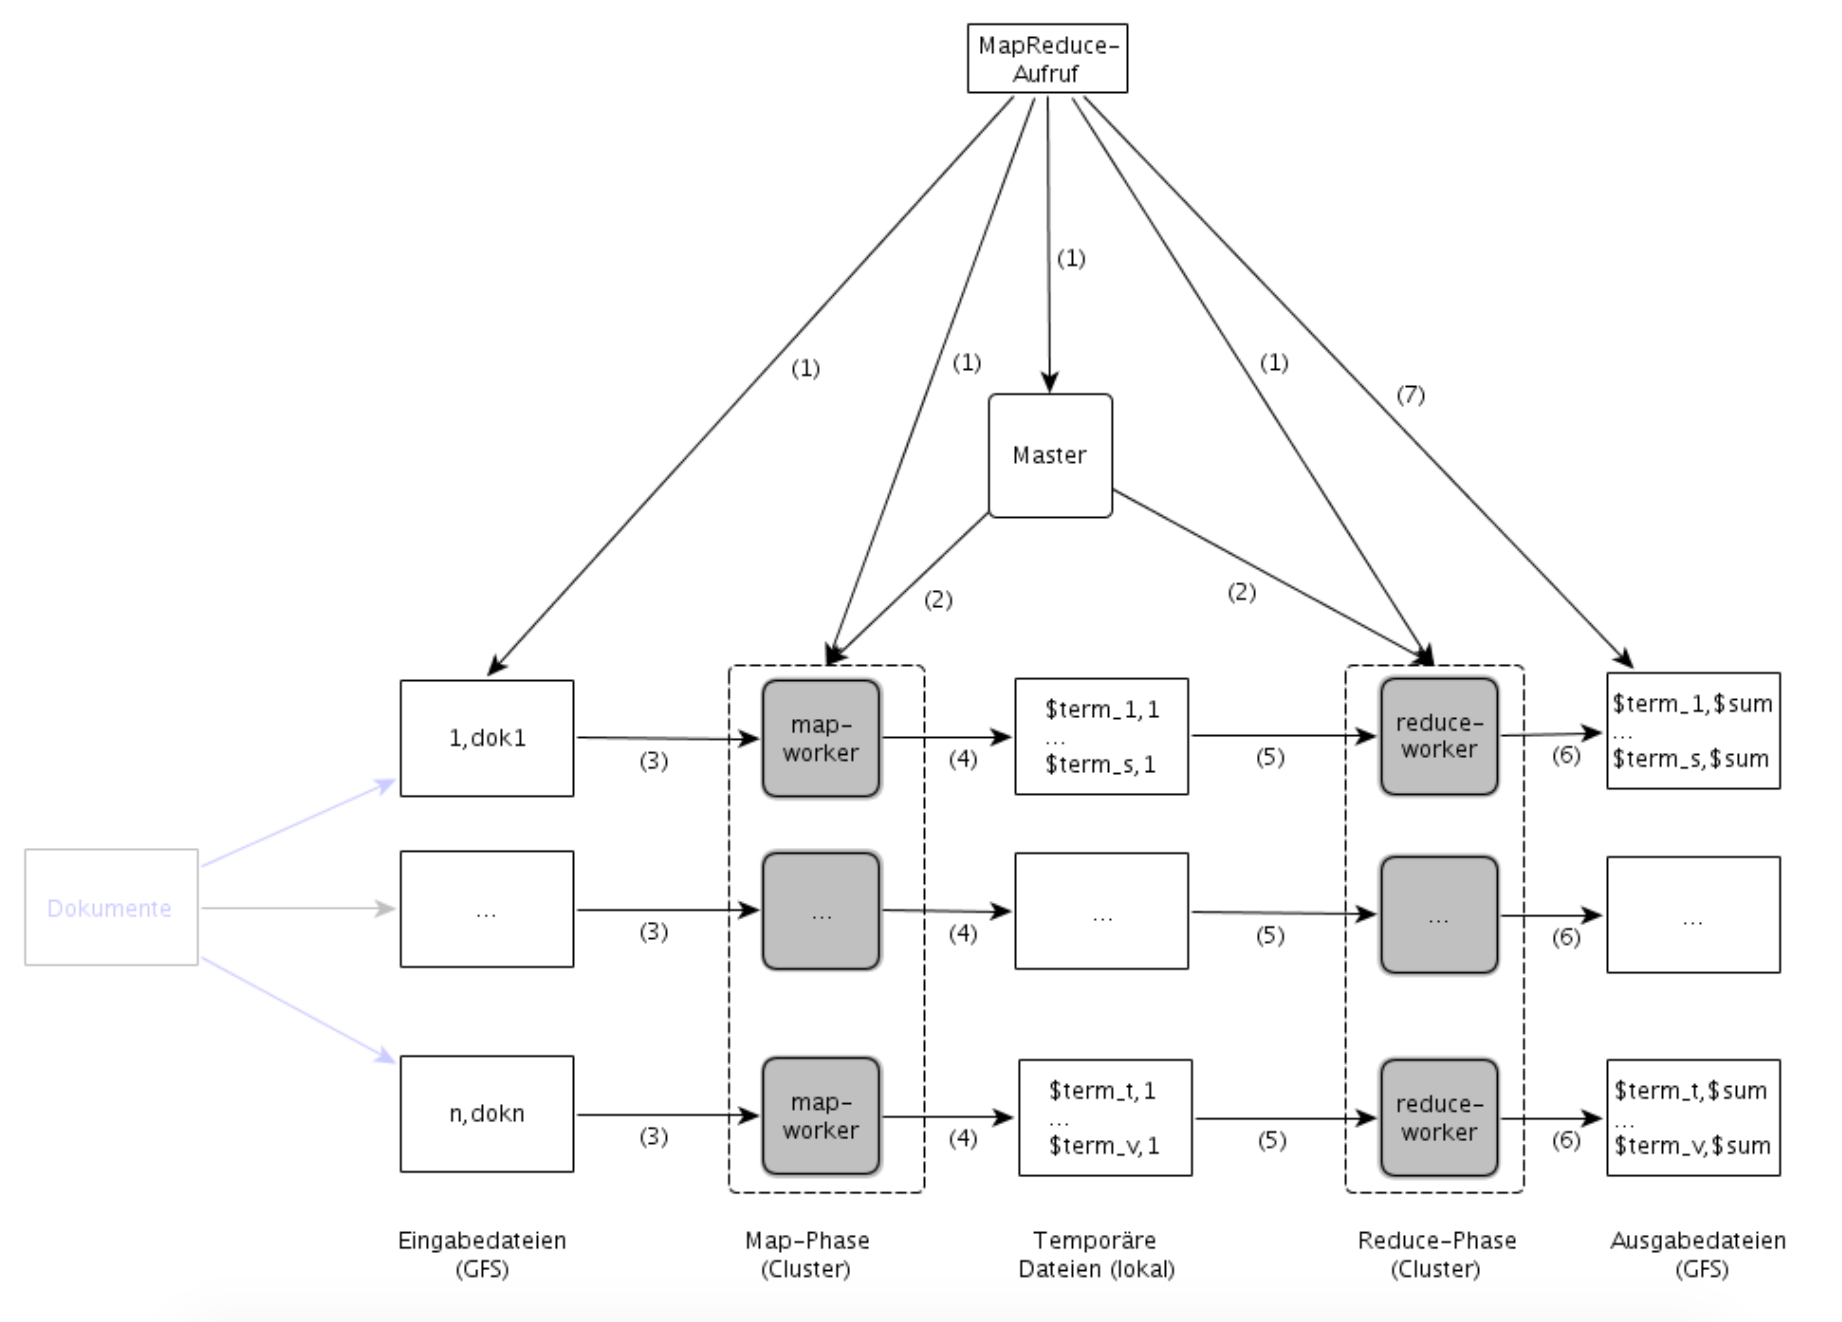
\includegraphics[width=0.9\textwidth]{picture/map_reduce_system_example.png}
	\caption{Systemübersicht eines Map-Reduce System \cite{Bethge2009}}
	\label{graphicMapReduceSystem}
\end{figure}

Weiterhin ist auf Abbildung~\ref{graphicMapReduceSystem} in Schritt 3 zu erkennen, dass jeder Worker, der eine Map-Aufgabe ausführt, eine Teilmenge der zu verarbeitenden Gesamtdatenmenge als Eingabe erhält. Die Daten müssen dazu in Form von Schlüssel-Wert Paaren gespeichert sein. Diese werden dann gemäß der vom Nutzer spezifizierten UDF verarbeitet. Als Ausgabe werden keine, ein oder mehrere Schlüssel-Wert Paare durch die map-Funktion produziert und im lokalen Festspeicher der jeweiligen Worker gespeichert. Aufgrund der Aufteilung der Gesamtdatenmenge in kleinere, von einander unabhängig prozessierbare Mengen, kann die Map-Phase parallelisiert ablaufen. Dabei werden auf jedem Worker des Clusters verschiedene Teilmengen der Eingabedaten verarbeitet. 

Nach Beendigung der Map-Phase folgt die Shuffle-Phase, auch Repartitionsphase genannt. Diese ist in Abbildung~\ref{graphicMapReduceSystem} als Schritt 4 gekennzeichnet. Während dieser werden die durch die Map-Funktion produzierten Schlüssel-Wert Paare gemäß ihrer Schlüssel vorerst partiell gruppiert. Wenn der Speicherbedarf für alle Schlüssel-Wert Paare einer Gruppe größer ist als der verfügbare Speicher auf einem Worker werden mehrere partielle Gruppen mit demselben Schlüsselwert gebildet. Jede partielle Gruppe wird anschließend in Schritt 5 auf verfügbare Worker übertragen und dort zu einer globalen Gruppe zusammen gefügt. \textcolor{red}{Ist wirklich Phase 5 die Shuffle Phase? Ich lese meine Quelle so, dass Phase 5 die Verteilung der repartionierten Gruppen an die Worker ist. Quelle: http://www2.informatik.hu-berlin.de/~bethge/public/MapReduce/document.pdf}

Die in Schritt 6 dargestellte reduce-Funktion wird dann auf jede in der Shuffle-Phase erzeugte globale Gruppe von Schlüssel-Wert Paaren angewendet. Die spezifizierte UDF wird auf die Werte aller Schlüssel-Wert Paare einer Gruppe angewendet. Als Ausgabe wird entweder keine, ein oder mehrere Schlüssel-Wert Paare produziert. 

Die Gesamtausgabe des Map-Reduce Programms besteht aus allen durch reduce-Funktionen produzierten Schlüssel-Wert Paaren.

Aufgrund der sehr genau festgelegten Programmstruktur, die zur Nutzung von Map-Reduce eingehalten werden muss wird der Anwender gezwungen einen Datenverarbeitungsprozess auf mehrere aufeinanderfolgende Map-Reduce Instanzen zu verteilen, wenn dieser zu komplex ist. 
 
Seit seiner Einführung im Jahr 2004 wurde das Map-Reduce Paradigma erweitert und bietet nun mehr Flexibilität, da es um weitere Funktionen zweiter Ordnung ergänzt wurde, die zusätzliche Datentransformationen ermöglichen. Aufgrund des Einsatzes von Map-Reduce in Hadoop \cite{HadoopWebsite} und anderen Systemen wie beispielsweise Spark \cite{Zaharia2010} bleibt es aber eines der dominanten Paradigmen bei der Verarbeitung großer Datenmengen. Auch Apache Flink \cite{FlinkWebsite} nutzt eine ähnliche Funktionsweise, um die parallelisierten Datenströme zu verwalten.

%Andere Systeme (Hadoop, AsterixDB, Spark etc)
Neben den bereits erwähnten Systemen Apache Hadoop und Apache Flink existieren weitere populäre Systeme, beispielsweise Apache Spark \cite{SparkWebsite, Zaharia2010}, Apache Storm \cite{StormWebsite, Jones2013} oder Asterix \cite{AsterixWebsite, Alsubaiee2012}. Diese unterscheiden sich bereits in ihrer Architektur. Während Apache Hadoop das Map-Reduce Paradigma sehr fixiert umsetzt und somit dem Nutzer nur eingeschränkte Mittel zur Spezifizierung seines Programmes lässt, setzen Systeme wie Apache Spark und Apache Flink das Map-Reduce Paradigma flexibler ein. Nachfolgend wird ein kurzer Überblick über die Funktionsweise der genannten Systeme gegeben. 

\textbf{Apache Hadoop}. Apache Hadoop implementiert das Map-Reduce System im Rahmen eines freien Projekts. Dabei können sowohl die Map- als auch die Shuffle- und Reducephase vom Nutzer individuell konfiguriert werden. Als freier Ersatz für GFS nutzt Hadoop das Dateisystem Hadoop Distributed File System (HDFS). In der Basisversion ermöglicht Hadoop lediglich Stapelverarbeitungen, echtzeitnahe Datenverarbeitung ist nicht vorgesehen. Hadoop wird in diversen Firmen genutzt, zum Beispiel verwendet Facebook das System zur Analyse von Datenmengen von bis zu 100 Petabyte \cite{Borthakur2013}.

\textbf{Apache Spark}. Apache Spark ist eine allgemeine Datenverarbeitungsplattform. Es beinhaltet mehr Funktionen zweiter Ordnung als Hadoop, es gibt also mehr Möglichkeiten verschiedene Datentransformationen auszuführen. Über den Funktionsumfang von Hadoop hinaus ermöglicht es neben der Stapelverarbeitung weitere Anwendungen wie zum Beispiel maschinelles Lernen. Des weiteren ist ebenfalls möglich Spark mit anderen Bibliotheken zu ergänzen. Diese Eigenschaften machen Spark gegenüber Hadoop für viele Anwendungszecke überlegen. 

\textbf{Apache Storm}. Apache Storm ist ein Datenverarbeitungssystem, das speziell auf die schnelle echtzeitnahe Verarbeitung von Daten ausgelegt ist. Ein Storm-Programm hat die Form eines direkten, azyklischen Graphs, dessen Kanten Datenströme darstellen. Ein Storm-Programm kann als datentransformierende Pipeline bezeichnet werden. Ein Storm-Programm entspricht einer Implementierung eines abstrakten Map-Reduce-Jobs. Im Unterschied zu einem Map-Reduce Job läuft ein Storm-Programm, bis es beendet wird. Dies unterstreicht den Einsatzzweck für echtzeitnahe Verarbeitung von Daten, die ohne Zeitbegrenzung generiert werden.

\textbf{AsterixDB}. AsterixDB ist ein \textit{Big Data Management System}, dass seit 2009 von den Universitäten Irvine, San Diego und Riverside gemeinschaftlich entwickelt wird. Das Ziel von AsterixDB ist eine effiziente parallelisierte Ausführung von Analysen auf semistrukturierten Daten. Dabei wird versucht Datenbanktechnologie mit Big-Data-Technologie zu kombinieren, um große Daten effizient verarbeiten zu können.

%Hadoop, z.b. bei 
\subsection{Apache Flink}
\label{sec:ApacheFlink}
%Flink einführen + allgemein beschreiben
Ein Datenverarbeitungssystem, das auf eine massiv parallelisierte Verarbeitung von großen Datenmengen spezialisiert ist, ist Apache Flink. Es ging 2014 aus Stratosphere hervor \cite{BraunWebsite}, einem Forschungsprojekt, das seit 2010 kooperativ von Forschern verschiedener Universitäten entwickelt wurde \cite{Battre2010, Alexandrov2014}. Seit Januar 2015 ist Apache Flink ein Top-Level Projekt der Apache Software Foundation \cite{ApacheFlinkBlogEntry}. 
Ähnlich wie andere Systeme ermöglicht es Apache Flink bereits vorhandene Daten in einem Stapel-Verfahren zu analysieren. Darüber hinaus können jedoch auch in Echtzeit zu verarbeitende Daten im Rahmen eines \textit{Streaming}-Verfahrens prozessiert werden. 

Die Hauptkomponenten von Apache Flink sind die Flink-Laufzeitumgebung (engl. \textit{Flink Runtime} ) und der Flink-Optimierer (engl. \textit{Flink Optimizer}). Darüber hinaus verfügt Flink über Programmierschnittstellen für die Hochsprachen Java, Python und Scala, mithilfe derer Nutzer Flink-Programme spezifizieren können. 

%Konzept: 2nd order functions, UDFs, Operatoren
Flink implementiert das vom Map-Reduce System bekannte Schema von Funktionen zweiter Ordnung und gekapselten nutzerdefinierten Funktionen erster Ordnung. Dabei beschreibt die Funktion zweiter Ordnung die Art der Datentransformation, die UDF definiert die vom Nutzer spezifizierte Verarbeitungslogik, die auf die Daten angewendet werden soll. Im Gegensatz zum Map-Reduce System verfügt Flink jedoch nicht nur über die Funktionen zweiter Ordnung Map und Reduce, sondern bietet insgesamt 15 verschiedene Datentransformationen. Diese werden als Operatoren bezeichnet. Weitere wichtige Operatoren sind neben Map und Reduce beispielsweise Cross, Match und CoGroup, die in der Grafik~\ref{graphicFlinkOperators} dargestellt sind. Die formalen Definitionen der Operatoren sind in Tabelle~\ref{tab:flinkOperatorsDefinition} aufgeführt. Nachfolgend werden die genannten Operatoren kurz beschrieben. Der \textit{Map}-Operator besitzt eine Eingabemenge und erstellt für jedes Element dieser Menge eine eigene Gruppe, die genau dieses Element enthält. Der \textit{Reduce}-Operator erstellt für jeden vorhandenen einzigartigen Schlüsselwert eine Gruppe und gruppiert alle Einträge mit demselben Schlüssel in dieselbe Gruppe ein. Der \textit{Cross}-Operator erstellt für jedes Eingabepaar von Werten aus zwei Eingabemengen eine Gruppe, die das kartesische Produkt der beiden Werte darstellt. Der \textit{Match}-Operator erstellt eine Gruppe für jedes Eingabepaar von Werten zweier Eingabemengen, genau dann wenn beide Werte denselben Schlüsselwert besitzen. Der \textit{CoGroup}-Operator erstellt für jeden einzigartigen Schlüsselwert, der in mindestens einer der beiden Eingabemengen enthalten ist, eine Gruppe und gruppiert in dieser alle Werte, die diesen Schlüsselwert aufweisen.
Jeder Operator besteht also aus jeweils einer spezifischen Transformation sowie einer eingebetteten UDF. Zusätzlich besitzen Operatoren eine Eingabe- sowie eine Ausgabedatenmenge in Form eines Datenstroms. Ein Flink-Programm wird als ein Datenfluss in Form eines direkten und azyklischen Graphen dargestellt, dessen Knoten Operatoren und dessen Kanten Datenströme darstellen. \textcolor{blue}{Ref auf Abbildung eines Beispieldatenstroms.}. Dieser wird \textit{Operator DAG} genannt. 

\begin{figure}[h]
	\centering	
	\captionsetup{justification=centering,margin=2cm}
	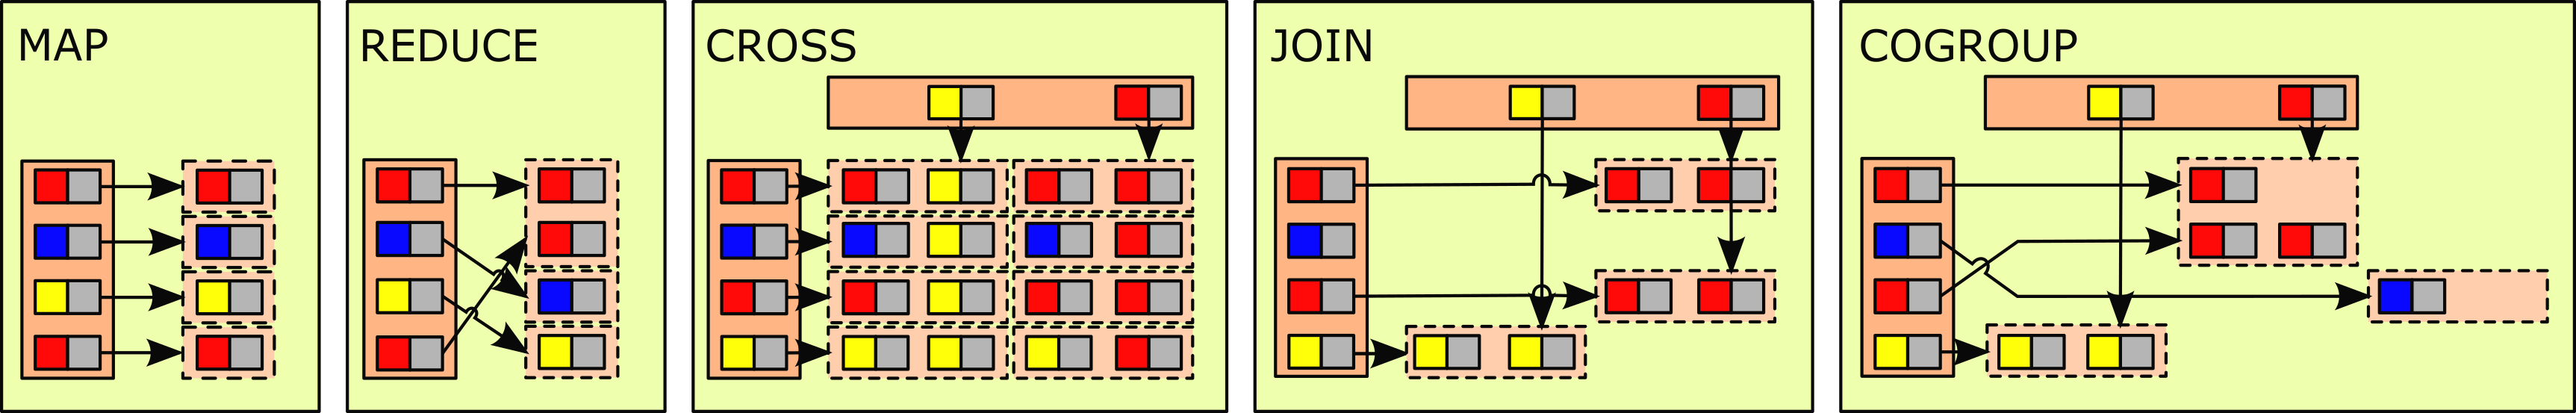
\includegraphics[width=0.9\textwidth]{picture/flink_operators.png}
	\caption{Funktionen zweiter Ordnung: (a) Map, (b) Reduce, (c) Cross, (d) Match und (e) CoGroup \cite{Hueske2012}}
	\label{graphicFlinkOperators}
\end{figure}

\begin{table}[position specifier]
          \centering
          \begin{tabular}{| c | C{12cm} |}
          	\hline
                  Operator & Formale Definition \\
                  \hline
                  Map & Map: \(\mathnormal{R} \times \mathnormal{f} \rightarrow [\mathnormal{f}(r_1),...,\mathnormal{f}(r_i),..,\mathnormal{f}(r_N)] \) \\
               
                  \hline
		Reduce & Reduce: \(\mathnormal{R} \times \mathnormal{f} \times \mathnormal{K} \rightarrow  [\mathnormal{f}(r_1^{k_1},..,r_{n_1}^{k_1}),...,\mathnormal{f}(r_i),..,\mathnormal{f}(r_N)] \) \newline mit \(\mathnormal{K}\) als Set von Schlüsseln \(\{k_1,...,k_l\} \) in \(\mathnormal{R}\) \\
                  \hline
                  Cross & Cross: \(\mathnormal{R} \times \mathnormal{S} \times \mathnormal{f} \rightarrow [\mathnormal{f}(r_1, s_1),\mathnormal{f}(r_1, s_2),..,\mathnormal{f}(r_N, s_M))] \) \\
                  \hline
                  Match & \(\mathnormal{R} \times \mathnormal{S} \times \mathnormal{K} \times \mathnormal{F} \times \mathnormal{f} \rightarrow [\{\mathnormal{f}(r, s)| r.K = s.F \}] \) \newline mit \(\mathnormal{K} \) und \(\mathnormal{F} \) als Schlüssel für \(\mathnormal{R} \) und \(\mathnormal{S} \). \\
                  \hline
                  CoGroup & \(\mathnormal{R} \times \mathnormal{S} \times \mathnormal{K} \times \mathnormal{F} \times \mathnormal{f} \rightarrow [\mathnormal{f}(r^{v_1}_1,...,r^{v_1}_{n_1},s^{v_1}_1,...,r^{v_1}_{m_1}),...,\mathnormal{f}(r^{v_l}_1,...,r^{v_l}_{n_l},s^{v_l}_1,...,r^{v_l}_{m_l})] \) \newline mit \(\{v_1,...,v_l\}\) als aktive Domain von \( \mathnormal{K}\) und \( \mathnormal{F}\) \\
                  \hline
          \end{tabular}
          \caption{Formale Definition der Operatoren Map, Reduce, Cross, Match und CoGroup mit den Eingabedatenmengen \(\mathnormal{R}\) = \([r_1,...,r_i,...,r_N]\), \(\mathnormal{S}\) = \([s_1,...,s_i,...,s_N]\) und \(\mathnormal{f}\) als UDF für die jeweilige Transformation. \cite{Hueske2012}}
          \label{tab:flinkOperatorsDefinition}
\end{table}

%Optimizer
Der Flink-Optimierer erhält den mithilfe einer Programmierschnittstelle spezifizierten Operator DAG als Eingabe. Die Aufgabe des Flink-Optimierers ist die Umwandlung des Operator DAG in einen parallelisiert ausführbaren Datenfluss, den \textit{OptimizedPlan}. Dieser Datenfluss soll möglichst stark parallelisierbar sein, damit eine effiziente Verarbeitung durch die Flink-Laufzeitumgebung ermöglicht werden kann. Um einen solchen Datenfluss zu erhalten werden abhängig von den verwendeten Operatoren programmspezifische Optimierungen vorgenommen. Dabei wird für jeden Operator auf Basis seiner Eingabedaten festgelegt, mit welcher internen Implementierung der Operator ausgeführt wird. Ein Beispiel dafür wäre die Ausführung eines Join-Operators wahlweise als Sort-Merge-Join oder als Hash-Join. Weitere Optimierungen umfassen die Wahl des Datenaustauschs zwischen den Operatoren sowie die Auswahl der Programmpunkte, an denen Zwischenergebnisse gespeichert werden. Außerdem wird versucht Daten, die durch einen Operator sortiert oder partioniert wurden, mit derselben Sortierung weiterzuverwenden, um weitere Sortier- oder Partionierungsprozesse zu vermeiden. Ist der optimale Datenflussgraph ermittelt, wird er zu einem \textit{JobGraph}, einem direkten azyklischen Graphen bestehend aus Operatoren und Zwischenergebnissen als Knoten, umgewandelt. Zur Ausführung durch die Flink-Runtime wird dieser Graph in einen \textit{ExecutionGraph} umgewandelt. Ein Bespiel für einen JobGraph sowie einen ExecutionGraph wird in Abbildung~\ref{graphicJobExecution} gezeigt. 

\begin{figure}[h]
	\centering
	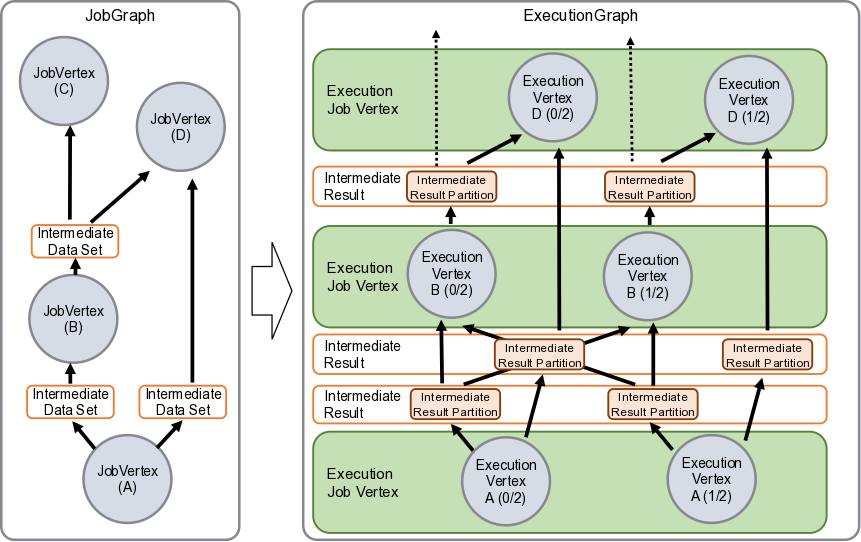
\includegraphics[width=0.9\textwidth]{picture/flink_job_and_execution_graph.png}
	\caption{Modell eines Jobgraphs und des dazugehörigen ExecutionGraphs \cite{FlinkJobWebsite}}
	\label{graphicJobExecution}
\end{figure}

%Konzept: JobManager: Masternode <-> Workernodes. Wie funktioniert die Parallelität?
Flink nutzt ebenso wie das Map-Reduce System eine Master-Worker Architektur zur Organisation des Netzwerkes, auf dem das Flink-Programm ausgeführt wird. Dementsprechend verwaltet der Master-Knoten, auch \textit{Jobmanager} genannt, eine variable Anzahl an Worker-Knoten, \textit{TaskManager} genannt. Diese TaskManager verfügen jeweils über eine variable Anzahl von \textit{TaskSlots}, die die Anzahl der parallel ausführbaren Prozesse festlegt. Analog zum Map-Reduce-System koordiniert der JobManager die Zuweisung der zu bearbeitenden Teilaufgabe des ExecutionGraph an die assoziierten TaskManager, die diese dann ausführen. Darüber hinaus werden die Funktionsfähigkeit der TaskManager sowie der Status jeder auszuführenden Teilaufgabe durch den JobManager überwacht. Im Falle eines Ausfalls eines TaskManagers werden dessen Aufgaben von anderen Worker-Knoten übernommen bzw. wiederholt. Im Gegensatz zum ursprünglichen Map-Reduce-System ist ein Datenaustausch zwischen den TaskManagern in Form von \textit{Data Streams} möglich. 

Bei der Ausführung eines Flink-Programms wird nach der Optimierung des Operator DAGs das System gemäß nutzerdefinierter Prämissen wie zum Beispiel dem Grad der Parallelität initialisiert. Der JobManager erhält den vom Flink-Optimizer generierten JobGraph als Eingabe. Dieser wird, wie in Abbildung~\ref{graphicJobExecution} dargestellt, in einen parallel strukturierten \textit{ExecutionGraph} transformiert. Für jeden Knoten des Jobgraphs wird ein \textit{ExecutionJobVertex} erstellt. Dieser verantwortet die Ausführung des durch den Knoten repräsentierten Operators sowie die Weitergabe der, aus der Anwendung des Operators auf die Eingabedaten resultierenden, Zwischenergebnisse. Dabei werden \textit{n ExecutionVertices} genutzt, wobei \textit{n} dem vom Nutzer festgelegten Grad der Parallelität entspricht. Jeder ExecutionVertex übernimmt die Ausführung einer der parallelisierten Verarbeitungsinstanzen des Operators. Dazu wird ein vom JobManager bestimmter Worker-Knoten genutzt. Der ExecutionJobVertex garantiert die komplette Ausführung des Operators auf der gesamten Eingabedatenmenge, indem der Status jedes ExecutionVertex verfolgt wird. Sollte einer der ExecutionVertices ausfallen wird die gerade verarbeitete Ausführungsinstanz an andere ExecutionVertices delegiert. Darüber hinaus beinhaltet der ExecutionGraph die Zwischenergebnisse, die zwischen der Anwendung verschiedener Operatoren erstellt werden. Dadurch ist jederzeit bekannt, ob die Bedingungen für die Ausführung eines weiteren Operators gegeben ist, oder ob noch nicht alle Eingabedaten in Form von Zwischenergebnissen verfügbar sind.

\subsection{Python}
\label{sec:Python}
Python ist eine höhere, interpretierte Programmiersprache, die seit 1989 existiert, quelloffen ist und fortwährend weiter entwickelt wird. Obwohl Python eine imperative Sprache ist, können auch objektorientierte und funktionale Programmierparadigmen verwendet werden. Jedes Python-Programm wird bei der Ausführung mittels des Python-Interpreters in Bytecode umgewandelt. Dieser ist plattformunabhängig lauffähig, so dass Python-Programme ohne weitere Modifizierung auf mehreren Systemen ausführbar sind. Eine weitere Eigenschaft von Python sind die sehr umfangreiche Standardbibliothek sowie die Erweiterbarkeit um Module und Bibliotheken. Des weiteren gibt es mit der Python-API die Möglichkeit Python-Code durch C- beziehungsweise C++-Bibliotheken zu erweitern \cite{Martelli2006}. Unter anderem aufgrund der maschinennahen Umsetzung und der effizient implementierten Compiler von C beziehungsweise C++ besitzen diese Sprachen einen Leistungsvorteil gegenüber anderen höheren Programmiersprachen. Dies kann in Python genutzt werden, indem leistungsintensive Programmteile direkt als C- oder C++-Code eingebunden und ausgeführt werden. Ein weiterer Vorteil von Python ist die starke Typisierung und daraus resultierend die bessere Optimierung des Codes bei der Übersetzung durch den Python-Interpreter. Zusätzlich nutzt Python Duck-Typing, also die Typbeschreibung eines Objekts alleinig durch das Vorhandensein bestimmter Methoden beziehungsweise Attribute, was die Nutzbarkeit der Typisierung durch den Entwickler vereinfacht.

Ein Schwachpunkt von Python im Bezug auf die schnelle Verarbeitung großer Datenmengen ist die nicht auf automatisierte Parallelisierung ausgelegte Architektur. Daraus resultiert eine unzureichende Skalierbarkeit der Datenverarbeitung, sobald Daten, deren Größe die Arbeitsspeichergröße der ausführenden Maschine übersteigt, verarbeitet werden müssen. Dies ist insbesondere im Zuge der in Abschnitt~\ref{sec:GrosseDatenmengen} aufgezeigten Entwicklung hin zu größeren zu verarbeitenden Datenmengen relevant. Entwicklungen, die eine bessere Parallelisierung und damit einhergehend eine bessere Skalierbarkeit von Python Projekten zum Ziel haben, sind jedoch meist nicht universal anwendbar oder bieten nicht den Funktionsumfang von Big-Data Systemen \cite{ParallelPythonWebsite, DispyWebsite}. Die Funktionalität dieser Entwicklungen wird dabei durch Module bereitgestellt, da sie nicht als Grundfunktion in Python existiert sondern projektweise hinzugefügt werden muss. Dies erhöht den zu leistenden Anpassungs- und Entwicklungsaufwand im Vergleich zu anderen Systemen, die mit Rücksicht auf diese Anwendungsfälle konzipiert wurden.

Trotzdem nutzen viele Anwender, die Big-Data Anwendungen entwickeln, Python \cite{Millman2011}. Einerseits ist die Sprache ein seit vielen Jahren bewährtes Werkzeug \cite{Beazley2000, Oliphant2007}, das durch Nutzung von Bibliotheken wie SciPy und NumPy effizient implementierbare Algorithmen ermöglicht, ohne dass alle genutzten Funktionen selbst programmiert werden müssen. Weitere Gründe für das Festhalten an Python sind zum Beispiel die Möglichkeit zur Einbindung von Fortran und die bei Nutzung neuerer Systeme notwendige Reimplementation bereits existierender Lösungen. Die Kosten-Nutzen-Relation bei einer Nutzung anderer Systeme wie zum Beispiel Apache Flink muss aufgrund des nötigen Entwicklungsaufwands projektabhängig und individuell aufgestellt werden. 

\subsection{Vergleichsmetriken}
\label{sec:Vergleichsmetriken}
%Einleitung, Aufzählung Kriterien
Um die Leistungsfähigkeit der verschiedener Systeme beziehungsweise Programmiersprachen vergleichen zu können, müssen Vergleichsmetriken definiert werden. Diese umfassen verschiedene Leistungskriterien, hinsichtlich derer die Systeme verglichen werden. Kriterien sind zum Beispiel die Datenverarbeitungsgeschwindigkeit, die Skalierbarkeit sowie das Verhältnis vom Preis zur Performance einer Anwendung. Einerseits kann eine offene Messung ohne Bezugswerte vorgenommen werden, die alle gemessenen Systeme untereinander vergleicht. Andererseits können Systeme hinsichtlich eines Referenzsystems evaluiert werden. Um die zu vergleichenden Kriterien mehrerer Varianten einer Anwendung auf verschiedener Systemen mit einem Referenzsystem vergleichen zu können, muss für jedes dieser Kriterien ein Referenzwert des Referenzsystems existieren. Dieser fungiert als Vergleichswert für alle Werte, die für die zu vergleichenden Anwendungsvarianten hinsichtlich dieses Kriteriums gemessen werden. Anhand der Unterschiedlichkeit von Mess- und Bezugswert kann das zu evaluierende System mit dem Bezugssystem verglichen werden. Hauptkriterium für traditionelle Datenbanksysteme ist die Datenverarbeitungsgeschwindigkeit, die als Durchsatzmetrik in Form von Arbeit pro Zeit definiert ist \cite{Gray1992}. Für diese Evaluation werden standardisierte Benchmarks verwendet, etwa TPC-H. Für Big-Data Anwendungen existiert darüber hinaus ein weiteres wichtiges Leistungskriterium, die Skalierbarkeit des Systems. Bis zum aktuellen Zeitpunkt hat sich allerdings noch kein standardisierter Benchmark für Big-Data Systeme etabliert. Jedoch werden bereits seit mehreren Jahren die Entwicklung solcher Benchmarks vorangetrieben \cite{Chen2014}. Ein Big-Data Benchmark muss dabei die Kriterien Datenverarbeitungsgeschwindigkeit, Skalierbarkeit sowie Preis/Performance evaluieren und auf sämtlichen Big-Data Systemen ausführbar sein \cite{Baru2013}.

%Kriterium Skalierbarkeit
Aufgrund des in Sektion~\ref{sec:BigData} beschriebenen Notwendigkeiten für parallele Datenverarbeitung vergrößern sich auch die zu verarbeitenden Datenmengen kontinuierlich. Deshalb ist die \textbf{Skalierbarkeit} des datenverarbeitenden Systems für Big-Data Anwendungen besonders wichtig, damit das Datenverarbeitungssystem flexibel auf die zu verarbeitende Datenmenge angepasst werden kann. Aufgrund ihrer parallelisierten Architektur, die aus mehreren miteinander verbunden Maschinen besteht, sind weitere Maschinen teilweise sehr einfach integrierbar. Sie müssen häufig lediglich an die bestehende Netzwerkinfrastruktur des Systems angeschlossen werden. Bei sequentiell arbeitenden Datenverarbeitungssystemen ist die Skalierbarkeit des Systems erschwert, da lediglich einzelne, geeignete Teilprozesse eines sequentiellen Programms manuell parallelisiert werden können. Darüber hinaus muss auch der Umgang mit Ausfällen der genutzten Hardware betrachtet werden. Im Idealfall wird der Ausfall von Netzwerkknoten wie bereits beim Map-Reduce System automatisiert isoliert und die Neuberechnung von Teilergebnissen auf ein notwendiges Minimum reduziert. Dieses Minimum entspricht dabei der Anzahl der notwendigen Neuberechnungen, die benötigt werden, um die Korrektheit der Ergebnisse zu garantieren. Das Ersetzen von fehlerhafter Hardware ist bei sequentiell arbeitenden Programmen meist nicht möglich, ohne die Anwendung abzubrechen. \textcolor{red}{Ist das richtig?}

%Kriterium Ausführungsgeschwindigkeit
Die Skalierbarkeit hat auch unmittelbare Folgen für die weiteren Bewertungskriterien, insbesondere für die \textbf{Datenverarbeitungsgeschwindigkeit} einer Anwendung. Aufgrund der Definition der Datenverarbeitungsgeschwindigkeit durch das Verhältnis von geleisteter Berechnungsarbeit pro Zeiteinheit sinkt sie bei einer Erweiterung der Rechenkapazitäten, wenn die Anwendung skaliert. Denn dementsprechend steigt die geleistete Berechnungsarbeit pro Zeiteinheit, was gleichbedeutend zu einer Beschleunigung der Datenverarbeitung ist. Die absolute Ausführungszeit einer Anwendung ist dabei das Produkt der Datenmenge und der Datenverarbeitungsgeschwindigkeit. Wächst die zu verarbeitende Datenmenge an, steigt demzufolge auch der nötige Verarbeitungsaufwand. Unter der Annahme einer identischen Datenverarbeitungsgeschwindigkeit steigt in diesem Fall auch die Ausführungsgeschwindigkeit. Aufgrund der im Allgemeinen wachsenden zu verarbeitenden Datenmengen muss die zur Verfügung stehende Rechenleistung erhöht werden, um die Datenverarbeitungsgeschwindigkeit und damit die Ausführungszeit einer datenverarbeitenden Anwendung zu verringern. Die Skalierbarkeit eines Big-Data Systems ist also essentiell für eine Datenverarbeitung mit gleicher Ausführungszeit bei wachsenden Datenmengen.

%Kriterium Preis/Performance
Obgleich die beiden genannten Kriterien die Leistungsfähigkeit eines Big-Data Systems definieren, muss zusätzlich der Preis des Systems im Verhältnis zur erzielten Datenverarbeitungsgeschwindigkeit betrachtet werden. Denn andernfalls wäre ein Leistungsvergleich von verschiedenen Datenverarbeitungssystemen nicht machbar, da etwaige Nachteile eines Systems durch zusätzliche oder bessere und somit teuerere Hardware ausgeglichen beziehungsweise verschleiert werden könnten. Aufgrund der Nutzung von Clustern von handelsüblicher Maschinen in verteilten Systemen sind diese meist günstiger als einzelne Maschinen die eine gleichwertige Rechenleistung aufweisen.

%----------------------------------------------------------------------------------

\chapter[Algorithmus zur Analyse von Pixelzeitreihen]{Beschreibung und Umsetzung des Algorithmus zur Analyse von Pixelzeitreihen}
\label{cha:AlgorithmForSatellitePictureAnalysis}
\section[Beschreibung des Algorithmus]{Beschreibung des Algorithmus zur Analyse von Pixelzeitreihen}
\label{sec:DescriptionOfTheAlgorithm}
%Einleitung: Kurze, grobe Beschreibung des Algorithmus, kurze Wiederholung relevante Geographische Grundlagen.
Das Ziel des in dieser Bachelorarbeit implementierten und evaluierten Algorithmus ist die Erkennung einer unerwarteten Veränderung der bewaldeten Fläche einer geographischen Region. Der Grad der Bewaldung wird dabei durch einen Vegetationsindex dargestellt. Um eine Veränderung dieses Indexes zu messen, werden die durch Landsat Satelliten aufgezeichneten Szenen der Zielregion dahingehend analysiert. Auf Basis dieser Analyse der in der Vergangenheit gemessenen Werte können dann zukünftige Indexwerte prognostiziert werden und etwaige Abweichungen des zukünftig tatsächlich gemessenen Vegetationsindexes automatisiert ermittelt werden. Die zu diesem Zweck eingesetzte Analyse ist eine Anwendung der \textit{Support Vector Regression} (SVR) \cite{Basak2007}, die in Abschnitt~\ref{subsec:svr} beschrieben wird. Die Ergebnisse der Analyse werden dann im Rahmen des \textit{Continuous Monitoring of Forest Disturbance Algorithm} (CMFDA) \cite{Zhu2012} genutzt. Dieser wurde 2012 von Zhu et al. vorgestellt \cite{Zhu2012} und wurde entwickelt, um die Veränderung von Waldbeständen geographischer Regionen kontinuierlich zu überwachen und atypische Veränderungen zu entdecken. 

%Beschreibung Vorbereitung: DataCubeCreation als Ausgangspunkt!, Schneiden der Szene in SlicedTiles, Gruppieren und sortieren.
Die in Algorithmus~\ref{alg:generalAlgorithm} beschriebene Vorgehensweise zeigt die Analyse der Veränderung des Vegetationsindexes der Pixel einer geographischen Region. Dieser Algorithmus benötigt eine Menge von Landsat-Szenen $S$ sowie die Koordinaten der Zielregion als Eingabe. Die genutzten Szenen beinhalteten dabei möglicherweise Daten von mehreren Spektralbändern. Die Szenen werden in Zeile~\ref{alg:groupOriginalScenes} zunächst gemäß ihres Aufnahmedatums $t \in T$ gruppiert. Mithilfe der Schleife in Zeile~\ref{alg:cutAllTilesOfAGroup} wird aus jeder Szene $s_t \in S$ die exakte Zielregion ausgeschnitten. Dieser Schritt ist notwendig, da etwaige Zielregionen zumeist kleiner sind als eine ursprüngliche Landsat-Szene oder nur ein Teil der Zielregion tatsächlich in der Ausgangsszene abgebildet ist. Der ausgeschnittene Bereich wird als Kachel $k_{t, b}$ bezeichnet und wird durch ihr Spektralband $b$ und den Aufnahmezeitpunkt $t$ charakterisiert. In Zeile~\ref{alg:groupTiles} werden anschließend alle Kacheln anhand ihrer Bänder gruppiert, so dass gilt $k_{t, b} \in K_{b} \forall k$. Um die Eigenschaften und Ordnung der Kacheln zu verdeutlichen, wird ein Würfel mit den Dimensionen Breite der Kachel, Höhe der Kachel und dem Aufnahmezeitpunkt der Kacheln modelliert. Dieser besteht aus den einzelnen nach $t$ sortierten Szenen, so wie in Abbildung~\ref{fig:dataCubeSliced} abgebildet. 

Jede Kachel $k_{t, b} \in K_{b}$ muss wie in Zeile~\ref{alg:sliceAllTiles} beschrieben in eine individuell festgelegte Anzahl von kleineren Kacheln, sogenannten Teilkacheln $tk_{t, pos\_tk, b}$, zerschnitten werden. Dabei werden zunächst aus Gründen der Vereinfachung nur quadratische Teilkacheln betrachtet. Dies impliziert, dass die Breite und die Höhe aller Kacheln $k \in K$ einen gemeinsamen Teiler besitzen müssen. Theoretisch ist aber auch die Nutzung von allgemein rechteckigen Teilkacheln möglich. Nachdem alle Kacheln $k_{t, b} \in K$ in Teilkacheln $tk_{t, pos\_tk, b}$ geschnitten wurden, werden diese gemäß ihrer geographischen Position sowie ihres Spektralbands gruppiert, so dass 

\begin{equation} \label{eq:numberOfSubsceneGroups}
tk_{t, pos\_tk, b} \in TK_{pos\_tk, b}\ \forall\ tk_{t, pos\_tk, b}
\end{equation}

 gilt. Die geographische Position ist in Abbildung~\ref{fig:dataCubeSliced} anhand der Tupel der Teilkacheln markiert, das als Wert für das Attribut $pos\_tk$ fungiert. Durch die Gruppierung aller Teilkacheln in Zeile~\ref{alg:groupSubscenes} entstehen 

\begin{equation} \label{eq:numberOfSubsceneGroups}
\text{ Anzahl von Teilkachelgruppen} = n \times b
\end{equation}

 verschiedene Gruppen von Teilkacheln mit $n$ = \{Anzahl der Teilkacheln pro Kachel\} und $b$ = \{Anzahl der betrachteten Spektralbänder\}. Im in Abbildung~\ref{fig:dataCubeSliced} gezeigten Beispiel werden drei Kacheln eines Bandes $b$ in jeweils 36 Teilkacheln unterteilt. Da $b=1$ ergeben sich gemäß der Formel~\ref{eq:numberOfSubsceneGroups} 36 Gruppen von Teilkacheln. Dabei sind alle Teilkacheln einer Gruppe $TK_{pos\_tk, b}$ durch das identische Positionstupel gekennzeichnet.

Jede dieser Gruppen wird dann in Zeile~\ref{alg:sortSubscenes} nach dem jeweiligen Aufnahmedatum der einzelnen Teilkacheln der Gruppe sortiert. 

\begin{figure}[H]
\centering
\includestandalone[width=9cm]{DataCubeSlicedImage}
\caption{Beispielhafte Kacheln gleicher Größe, ausgeschnitten aus Szenen $s_t \in S$. Die Tupel geben die Position $pos\_tk$ der Teilszenen innerhalb der Kachel an und werden als Gruppenschlüssel zum Gruppieren der Teilszenen verwendet.} 
\label{fig:dataCubeSliced}
\end{figure}

\begin{equation} \label{eq:pixelTimeSeries}
pts_{pos\_px} = \{P_{t_1, pos\_px, b}, ..., P_{t_i, pos\_px, b}, ... , P_{t_n, pos\_px, b}\} | t_1, ..., t_i, ..., t_n \in T
\end{equation}

Um die Veränderung des Vegetationsindex jedes betrachteten Pixels analysieren zu können, muss in Zeile~\ref{alg:createPixelTimeSeries} zunächst für jeden Pixel eine Pixelzeitreihe $pts_{pos\_px}$ gebildet werden, die gemäß Definition ~\ref{eq:pixelTimeSeries} strukturiert sind. Da die Gruppen der Teilkacheln $TK_{pos\_tk, b}$ nur die Pixelwerte eines Spektralbandes enthalten, gilt für alle Pixelzeitreihen implizit, dass sie nur die Pixelwerte eines Spektralbandes enthalten. Folglich muss bei der Konstruktion der Pixelzeitreihen keine weitere Unterscheidung nach diesem Kriterium erfolgen. In jeder Pixelzeitreihe $pts_{pos\_px} \in TK_{pos\_tk, b}$ ist jedem bekannten Vegetationswert $V_{pos\_px, t}$ genau ein fester Zeitpunkt $t \in T$ zugeordnet, zu dem der Wert durch die Auswertung des Pixelwerts des Satellitenbildes bekannt ist. Allerdings ist nicht jedem Wert $t$ für alle Positionen $pos\_px$ ein Wert $V_{pos\_px, t}$ zugeordnet, da die Eingabedaten entweder keine Szene $s_t$  enthalten oder der Pixel an der Stelle $pos\_px$ für das betrachtete Spektralband $b$ keinen validen Vegetationsindexwert enthält. Dies kann aufgrund externer Störfaktoren wie Wolken, Wolkenschatten oder Schnee zum Zeitpunkt der Aufnahme der Fall sein. Sollte der Wert für $V_{pos\_px, t}$ nicht verfügbar sein, wird der Aufnahmezeitpunkt $t$ aus Pixelzeitreihe entfernt. Auf Basis der vorhandenen Werte wird dann in Zeile~\ref{alg:approxPixelTimeSeries} mittels einer Regressionsanalyse eine Funktion approximiert, die die Werte für alle $t \in T$ bestmöglich annähert. Für die Regressionsanalyse wird das Regressionsverfahren Support Vektor Regression eingesetzt, das nachfolgend erklärt wird. \\

\begin{algorithm}[H]
\small
\caption{Analyse der Vegetationsveränderung einer geographischen Region}
\label{alg:generalAlgorithm}
\begin{algorithmic}[1]
\Function{ApproximateVegetationIndex}{$S, G$}
	\State \textbf{input:} Landsat-Szenen $S$, Zielregion $G$
	\State \textbf{output:} Teilkacheln mit approximierten Vegetationsindexwerten $V$ für jeden Pixel $P \in s\ \forall\ s \in S$
	\LineComment{Gruppiere alle Szenen gemäß dem Aufnahmezeitpunkt}
	\For{$s \in S$}
        		\State $S_t \leftarrow s_t $ \label{alg:groupOriginalScenes}
	\EndFor
	\LineComment{Schneide den Zielbereich aus den Szenen und gruppiere alle Kacheln gemäß ihrem Band}
	\ForAll{$S_t $} \label{alg:dataCubeCreation}
		\ForAll{$s_t \in S_t$}
			\State $k_{t, b} \leftarrow matching\ Region (s_t, G)$ \label{alg:cutAllTilesOfAGroup}
			\State $K_{b} \leftarrow k_{t, b}$ \label{alg:groupTiles}
		\EndFor
	\EndFor
	\LineComment{Schneide alle Kacheln in Teilkacheln und gruppiere alle Teilkacheln gemäß ihrer Position}
	\ForAll{$k_{t, b} \in K_{b}$} \label{alg:flatMapOperator}
		\State $Teilkacheln\ tk_{t, pos\_tk, b} \leftarrow zerschneide\ Kachel (k_{t, b})$ \label{alg:sliceAllTiles}
		\State $TK_{pos\_tk, b} \leftarrow tk_{t, pos\_tk, b}$ \label{alg:groupSubscenes}
	\EndFor
	\LineComment{Sortiere die Teilkachelgruppen nach Aufnahmezeitpunkt}
	\ForAll{$TK_{pos\_tk, b}$}
		\State $TK_{pos\_tk, b} \leftarrow\ sortiere\ \forall tk_{t, pos\_tk, b} \in TK_{pos\_tk, b}\ nach\ t$ \label{alg:sortSubscenes}
		\LineComment{Erstelle jeweils eine Pixelzeitreihe für jede Pixelposition in einer Teilkachelgruppe}
		\ForAll{$tk_{t, pos\_tk, b} \in TK_{pos\_tk, b}$} \label{alg:createPixelTimeSeriesLoopStart}
			\ForAll{$P_{pos\_px} \in tk_{t, pos\_tk, b}$}
				\State {$Pixelzeitreihe\ pts_{pos\_tk} \leftarrow P_{pos\_px}$} \label{alg:createPixelTimeSeries}
			\EndFor
		\EndFor \label{alg:createPixelTimeSeriesLoopEnd}
		\LineComment{Approximiere alle Pixelzeitreihen der Teilkachelgruppe}
		\ForAll{$pts_{P\_}$}
			\State {$pts_{P} \leftarrow approximiere\ fehlende\ V_{p, t} \forall p \in P \in pts{P}$} \label{alg:approxPixelTimeSeries}
		\EndFor
	\EndFor
\EndFunction

\end{algorithmic}
\end{algorithm}

\subsection{Support Vektor Regression}
\label{subsec:svr}
%Beschreibung SVR
Die Support Vector Regression ist ein Regressionsverfahren, das auf \textit{Support Vector Machines}, auch Stützvektormaschinen genannt, aufbaut \cite{Drucker97}. Support Vector Machines bezeichnen ein mathematisches Verfahren zur Mustererkennung, das seine Ursprünge im maschinellen Lernen hat. 

\begin{equation} \label{eq:svrFormula}
\{{(x_1, y_1)},...,{(x_n, y_n)}\} \subset \chi \times \mathbb{R}
\end{equation}

Dabei wird für einen Trainingsdatensatz gemäß der Formel~\ref{eq:svrFormula}, wobei \(\chi\) die räumliche Dimension der Eingabedaten angibt, für jeden Beobachtungswert \(y_i \) ein Wert \( \hat{y}_i \) bestimmt. Die Distanz \( \epsilon \) zwischen \( y_i \) und \( \hat{y}_i \) wird durch \( \epsilon_i = | y_i - \hat{y}_i | \) berechnet. Um die Güte der Regression anzupassen, kann eine maximale Distanz $\bar{\epsilon}$ definiert werden. Bei der Annäherung der Funktion \(f(x) \) anhand der Beobachtungswerte $y$ werden nur Beobachtungswerte $y_i$ mit $\epsilon_i \leq \bar{\epsilon}\ \forall i$ berücksichtigt. Dadurch wird eine übermäßige Verzerrung der Regressionsfunktion durch statistische Ausreißer verhindert.

\begin{equation} \label{eq:minimizeW}
\min_{\omega} | \omega = \sum_{i=0}^{n} \epsilon_i\
\end{equation}

Um eine optimale Annäherung der Funktion \(f(x) \) und somit der approximierten Werte an die tatsächlichen Werte zu erhalten, muss \( f(x) \) so gewählt werden, dass die Summe der Abweichungen gemäß Formel~\ref{eq:minimizeW} minimal ist. 

\begin{figure}[H]
	\centering
	\begin{tikzpicture}[>=latex']
		\begin{axis}[xmin=0, xmax=6*pi, ymin=-2, ymax=2, xlabel={Zeit}, ylabel={Beobachtungswerte},legend style={ 
			at={(current bounding box.south-|current axis.south)},
  			anchor=north,
		},]
			\addplot [only marks, mark=x, color = blue] table {
				0.4   0.3
				1.1 0.5
				2.5  1.2
				3.4  -0.4
				4.9 -1.2
				6 1.8
				7.3  1.1
				8.2  0.5   
			};
			\addlegendentry{$Gemessene\ Pixelwerte$}
			
			\addplot [only marks, mark=x, color = red] table {
				0.4   0.39
				1.1 0.89
				2.5  0.59
				3.4  -0.26
				4.9 -0.98
				6 -0.28
				7.3  0.85
				8.2  0.94   
			};
			\addlegendentry{$Approximierte\ Pixelwerte$}
			
			\addplot[samples=500,domain=0:6*pi, color=green]{sin(deg(x))};
			\addlegendentry{$Approximierte\ Sinusfunktion$}
			
			\addplot[thin, samples=20, smooth,domain=0:6,magenta, name path=epsilon] coordinates {(0.4, 0.3)(0.4, 0.39)};
			\addplot[thin, samples=20, smooth,domain=0:6,magenta, name path=epsilon] coordinates {(1.1, 0.5)(1.1, 0.89)};
			\addplot[thin, samples=20, smooth,domain=0:6,magenta, name path=epsilon] coordinates {(2.5, 1.2)(2.5, 0.59)};
			\addplot[thin, samples=20, smooth,domain=0:6,magenta, name path=epsilon] coordinates {(3.4, -0.4)(3.4, -0.26)};
			\addplot[thin, samples=20, smooth,domain=0:6,magenta, name path=epsilon] coordinates {(4.9, -1.2)(4.9, -0.98)};
			\addplot[thin, samples=20, smooth,domain=0:6,magenta, name path=epsilon] coordinates {(6, 1.8)(6, -0.28)};
			\addplot[thin, samples=20, smooth,domain=0:6,magenta, name path=epsilon] coordinates {(7.3, 1.1)(7.3, 0.85)};
			\addplot[thin, samples=20, smooth,domain=0:6,magenta, name path=epsilon] coordinates {(8.2, 0.5)(8.2, 0.94)};
			\addlegendentry{$Distanz\ \epsilon$}
		\end{axis}
	\end{tikzpicture}
	\caption{Graphische Darstellung der Berechnung der Distanz $\epsilon$ zwischen gemessenen und approximierten Werten}
\end{figure}

Im Rahmen dieser Bachelorarbeit wird die SVR-Methode auf die einzelnen Pixelzeitreihen $pts_{pos\_px}$ angewendet. Dadurch werden für alle $P_{pos\_px, t} \in pts_{pos\_px}\ \forall\ pts_{pos\_px}$, für die kein Pixelvegetationsindexwert $V_{pos\_px, t}$ vorliegt, Werte auf Basis der vorhandenen Daten approximiert. Außerdem werden alle Werte, die die maximale Distanz $\bar{\epsilon}$ überschreiten, aus der Pixelzeitreihe gelöscht, da es sich höchstwahrscheinlich um nicht korrekte Werte handelt. Diese würden wenn sie weiterhin in der Pixelzeitreihe verbleiben würden die Güte der Analyse verschlechtern, da diese alle Beobachtungswerte betrachtet und bei der Bildung der Approximierungsfunktion berücksichtigt.

Nach der Anwendung der SVR-Methode enthält jede Pixelzeitreihe die Vegetationsindexwerte $V_{pos\_px, t}\ \forall\ t \in T$. 

Da die Güte der Approximierung durch bereits durchgeführte Experimente bereits bekannt und zufriedenstellend ist, kann auf einen Testdatensatz verzichtet werden.

\subsection{Komplexitätsanalyse}
\label{sec:ComplexityAnalysis}
Kurze Einleitung, Beschreibung meiner Kompl.A. (Big O Notation kurz erläutern)

Kompl.A. für den Algorithmus

\section{Umsetzung des Algorithmus mit Apache Flink}
\label{sec:ImplementationFlinkDescription}
%Kurze Einleitung - auf Ziel der Arbeit eingehen und kurz beschreiben, wie mit Flink gearbeitet wird
Der in Unterkapitel~\ref{sec:DescriptionOfTheAlgorithm} beschriebene Algorithmus wird im Rahmen dieser Arbeit in Apache Flink implementiert. Dazu werden die in Kapitel~\ref{sec:ApacheFlink} erwähnten Programmierschnittstellen für Java sowie Python genutzt. Grund für die Auswahl von Java sind die Stabilität und der Umfang der Java-Programmierschnittstelle von Flink. Die Motivation Python zu verwenden liegt darin begründet, dass viele Forscher Python zur Analyse von Daten nutzen und für die Analyse von Daten effizient implementierte Bibliotheken existieren, die viele wichtige Funktionen beinhalten. Diese Bibliotheken können auch bei der Nutzung von Python in Verbindung mit Flink weiterhin verwendet werden. Grundlage für beide Implementationen ist der vom Geographischen Institut der Humboldt-Universität zu Berlin umgesetzte Algorithmus, der in Python implementiert ist.

%Im Gegensatz dazu ist ein Python-Programm gemäß der Beschreibung in Kapitel~\ref{sec:python} ein dynamisch interpretiertes Programm, das sequentiell ausgeführt wird. Insofern muss die Struktur der vorhandenen Implementation an die von Flink benötigte Programmstruktur angepasst werden. 
Wie bereits in Kapitel~\ref{sec:ApacheFlink} beschrieben, sind Flink-Programme unabhängig von der verwendeten Programmierschnittstelle Datenströme, die aus Datenquellen, Datentransformationen und Datenausgaben bestehen. Der entsprechende Datenfluss-Graph, den das Flink-Programm beschreibt, ist in Abbildung~\ref{fig:dataFlowAlgorithm} abgebildet und wird für beide Implementationsvarianten verwendet. Die im nachfolgenden Abschnitt referenzierten Arbeitsschritte beziehen sich auf die mit den entsprechenden Nummern gekennzeichneten Datentransformationen. In Schritt 1 des Datenflusses stellt eine Datenquelle die zu analysierenden Satellitenbilder im .bsq Format mit zugehörigen .hdr Dateien, die Metadaten bezüglich der Szene beinhalten, zur Verfügung. Diese werden mithilfe eines Parsers eingelesen, der die einzelnen Szenen in Datenobjekte umwandelt. Diese verfügen über alle Attribute, die zur Beschreibung der Szene notwendig sind, darunter, das Aufnahmedatum, die Eckkoordinaten sowie ein Array der Vegetationsindexwerte. Um die Szenen für die spätere Analyse aufzubereiten, werden die erzeugten Datenobjekte in Verarbeitungsschritt Nummer 2 gemäß ihrem jeweiligen Aufnahmedatum gruppiert. Diese Gruppierung erfolgt durch die Anwendung der \textit{GroupBy}-Transformation, die alle Szenen als Eingabemenge hat und gemäß dem Schlüsselwert Aufnahmezeitpunkt $t$ in Gruppen $S_t | t \in T$ zusammengefasst ausgibt. Aus allen so gruppierten Szenen werden dann in Schritt 3 mithilfe einer \textit{groupReduce}-Funktion Kacheln zurecht geschnitten, die nur noch die für den durch den Nutzer bestimmten geographischen Bereich relevanten Teilszenen beinhalten. Aktuell muss dieser Bereich eine kleinere geographische Region abbilden als die Szenen der Eingabedatenmenge. Diese werden dabei außerdem gemäß ihrem Spektralband gruppiert, so dass die Schleife in Zeile~\ref{alg:dataCubeCreation} des Algorithmus~\ref{alg:generalAlgorithm} komplett implementiert ist. Die Kachel-Datenobjekte sind dabei identisch zu den Szenen-Datenobjekten aufgebaut, da eine Kachel lediglich eine Szene mit anderen Abmessungen ist. Für diese Arbeitsschritte wird eine bereits vorhandene Implementation verwendet.
Nachdem die Ausgangsszenen auf den relevanten geographischen Bereich reduziert wurden, werden alle Kacheln $k_{t, b} \in K_{b}$ in kleinere Teilkacheln $tk_{t, pos\_tk, b}$ zerschnitten. Dafür wird wie in Schritt 4 dargestellt der \textit{Flatmap}-Operators auf jede Kachel angewendet. Da alle Kacheln unabhängig voneinander verarbeitet werden, können alle FlatMap-Operationen in diesem Schritt parallelisiert ausgeführt werden. Die Teilkacheln werden dabei als Teilkachel-Datenobjekte umgesetzt, die alle Eigenschaften der Kachel-Objekte implementieren und zusätzlich über ein Positionsattribute verfügen. Damit alle Pixel in genau einer Teilkachel enthalten sind, muss die Bedingung~\ref{eq:conditionXEqualsY} gelten. Wäre dies nicht der Fall, würden bei der Anwendung der FlatMap-Operation Pixel verloren gehen. Dies bedeutet im Umkehrschluss, dass die Kantenlängen der ungeschnittenen Kacheln mindestens einen ganzzahligen Teiler besitzen müssen. Eine Alternative wäre das Zulassen von Rest-Teilkacheln, dann wäre die Bedingung~\ref{eq:conditionXEqualsY} nicht mehr notwendig. Das Erzeugen der Teilkacheln entspricht der Schleife in Zeile~\ref{alg:flatMapOperator} des Algorithmus~\ref{alg:generalAlgorithm}.

\begin{equation} \label{eq:conditionXEqualsY}
\text{Kantenlänge}_{Kachel} \bmod \text{Kantenlänge}_{Teilkachel} = 0
\end{equation}
 
Nachdem die Teilkacheln $tk_{t, pos\_tk, b}$ korrekt erzeugt wurden, werden sie wiederum gemäß ihrem Zeitstempel $t$ in Teilkachelgruppen $TK_{pos\_tk, b}$ gruppiert. Anschließend wird der \textit{Sort}-Operator genutzt, um alle Teilkacheln in den Teilkachelgruppen jeweils nach dem Aufnahmedatum $t$ der enthaltenen Teilkacheln zu sortieren. Dies ist notwendig, um die korrekte zeitliche Abfolge der Beobachtungen sicherzustellen, die bei der Analyse der Daten vorausgesetzt wird. Die Gruppierung und Sortierung entsprechen den Arbeitsschritten 5 und 6.
Nachdem die Teilkacheln auf diese Weise vorbereitet wurden, können die Pixelzeitreihen $pts_{pos\_tk}$, wie in den Zeilen~\ref{alg:createPixelTimeSeriesLoopStart} bis~\ref{alg:createPixelTimeSeriesLoopEnd} beschrieben, konstruiert werden. 
Diese erfolgt zusammen mit der Analyse durch die Anwendung des GroupReduce-Operators auf alle nach $t$ sortierten Gruppen von Teilkacheln $TK_{pos\_tk, b}$ wie in Schritt 7 beschrieben. Nachdem innerhalb der GroupReduce-Funktion die Pixelzeitreihen für die verarbeitete Teilkachelgruppe konstruiert wurden, wird die Analyse auf diese angewendet. Dazu wird wie in Kapitel~\ref{sec:DescriptionOfTheAlgorithm} beschrieben ein SVR-Modell konstruiert und gelöst, so dass die Vegetationsindexwerte $V_{pos\_px, t}$ ensprechend approximiert werden. 

Bei der Durchführung beider Analysen werden sowohl bei der Nutzung der Java- als auch bei der Nutzung der Python-Programmierschnittstelle von Flink teilweise externe Bibliotheken genutzt. Die Unterschiede bei der Nutzung der jeweiligen Bibliotheken werden in Sektion~\ref{sec:Differences} aufgezeigt. 

Nach der Durchführung der Analyseoperationen werden die Analyseergebnisse in Form eines 4-Tupels der Form $(Pixelposition_x, Pixelposition_y, Band, Ergebnisvektor\ \alpha)$ gemäß Schritt 8 in einer Textdatei gespeichert und in einer vom Nutzer zu spezifizierenden Ausgabedatei abgelegt.

\begin{figure}[h]
\centering
\includestandalone[width=8cm]{algorithmOperators}
\caption{Visualisierung des Datenstroms des Analysealgorithmus} 
\label{fig:dataFlowAlgorithm}
\end{figure}

%Minimal diagram example
%\begin{tikzpicture}[nodes=draw]
%    \node [label=label1,draw] (node1) {Node1};
%\end{tikzpicture}

\subsection{Unterschiede zwischen den drei Implementationsvarianten}
\label{sec:Differences}
%Muss enthalten: Python kann C Code, Python ist nicht typsicher -> Annotations, 
Die Implementation des Algorithmus als Apache Flink-Programm erfolgt über die Nutzung der jeweiligen Programmierschnittstellen, die für Java und Python zur Verfügung stehen. In beiden Varianten wird dabei der Datenstrom aus Abbildung~\ref{fig:dataFlowAlgorithm} umgesetzt. Aufgrund der Verschiedenheit der Sprachen Java und Python sowie der zugehörigen Schnittstellen sind die Implementationen nicht identisch, auch wenn sie prinzipiell denselben Algorithmus implementieren. Dies liegt hauptsächlich daran, dass die Spracheigenschaften von Python, die in Kapitel~\ref{sec:Python} beschrieben wurden, und Java unterschiedlich sind. Zusätzlich unterscheidet sich auch der Funktionsumfang der beiden Schnittstellen, was auch in der unterschiedlichen Spracheigenschaften begründet liegt. Diese Unterschiede müssen bei der Implementation berücksichtigt werden. 

Ein bedeutender Unterschied zwischen der Java- und der Python-Programmierschnittstelle ist die unterschiedliche Art des effizienten Speicherns von Objekten. Flink Java-Objekte werden mithilfe eingebauter Serialisierer beziehungsweise durch die Nutzung von Kryo in Byte Arrays umgewandelt, um die angelegten Objekte effizient im Speicher zu halten. Für Python-Objekte müssen hingegen für jedes Objekt eigene Serialisierer implementiert werden, die die Python-Objekte in Java-Objekte umwandeln. Dieser werden von Flink dann entsprechend serialisiert. Entgegen der Spracheigenschaft von Python, die eine dynamische Typisierung von Variablen vorsieht, müssen bei der Serialisierung alle Attribute der Objekte statisch typisiert sein. Auf diese Weise wird den Attributen eine Typinformation beigefügt, die es Flink erlaubt den Datentyp des Attributes zu erkennen. Basierend auf dieser Typinformation weist Flink bei der Speicherung der Daten jedem Attribut Speicherplatz in der dem Datentyp entsprechenden Größe zu. Da von der Python-Schnittstelle zur Zeit lediglich die Datentypen Integer, Float, Boolean, String sowie Byte Arrays unterstützt werden, müssen andere Datentypen vor der Serialisierung in akzeptierte Typen umgewandelt werden. Des weiteren muss für jeden Serialisierer auch ein Deserialisierer vorhanden sein, der die Java-Objekte wieder in Python-Objekte transformiert.

Wie bereits in Sektion~\ref{sec:Python} erwähnt, verfügt Python über die Möglichkeit Teile der Implementation in C statt in Python zu implementieren. Diese werden vom Python-Interpreter erkannt und direkt in C ausgeführt, was die Verarbeitungsgeschwindigkeit dieses Teils des Algorithmus steigern kann. Dementsprechend sind einige Teile der für die Regression genutzten Python-Bibliotheken NumPy und SciPy in C geschrieben und lediglich in Python eingebettet. Damit ermöglicht Python die Nutzung von Algorithmen, die möglicherweise schneller ausgeführt werden können als die entsprechenden Java-Implementationen. Dies ist nicht zwangsweise der Fall, da Java Just-in-time- Kompilierung unterstützt, das während der Ausführung der Java-Implementation Optimierungspotenzial durch Caching und ähnliche Techniken erkennt und entsprechend nutzt. Es soll Ziel der Untersuchungen dieser Bachelorarbeit sein, welche Variante bei der Anwendung des in Kapitel~\ref{sec:DescriptionOfTheAlgorithm} beschriebenen Algorithmus schneller ausgeführt wird.

Zusätzlich zu den Implementationen des Algorithmus in Apache Flink mittels der Java- bzw. der Python-Programmierschnittstelle wird eine weitere Implementierung in Python betrachtet. Die Implementation besitzt dabei die in Sektion~\ref{sec:Python} beschriebenen Vor- und Nachteile eines Python-Programms. Zwar lässt sich der Analysealgorithmus mithilfe von effizient umgesetzten Bibliotheken so umsetzen, dass die Berechnungszeit auf sequentiell arbeitenden Maschinen gut ist. Jedoch lässt sich das Programm nicht automatisiert parallelisieren, so dass der Algorithmus bei zunehmenden Datenmengen nur schlecht skaliert. 
Aufgrund der Charakteristika der Problemstellung, die eine Aggregation von Satellitenbildern fordert, wobei die Anzahl der Szenen sich fortlaufend erhöht und auch die Größe der Zielregion variabel ist, ist die mangelnde Parallelisierbarkeit problematisch. Vermutlich ist die Laufzeit des Algorithmus akzeptabel, solange die Eingabedatengröße die Größe des verfügbaren Hauptspeichers nicht überschreitet. Ist dies jedoch der Fall, verringert sich die Verarbeitungsgeschwindigkeit des Algorithmus, da die Eingabedaten direkt von einem langsameren Speicher als dem Hauptspeicher wie zum Beispiel einer Festplatte gelesen werden müssen. 
\newline
%Bei der Analyse von Satellitenbildern sind die Merkmale Datengröße und Datenkomplexität sowie die schnelle Verarbeitung der Daten von Bedeutung. Abhängig von der Anzahl der genutzten Bilder sind die zu verarbeitenden Datenmengen sehr groß. Ein Bild besitzt im Regelfall abhängig vom Satellitenmodell, das die Aufnahme gemacht hat, eine Größe von 750 Megabyte bis zu 1,5 Gigabyte. Um eine Entwicklung zu untersuchen werden jedoch viele dieser Bilder in die Untersuchung mit einbezogen, so dass die zu verarbeitende Datenmenge kontinuierlich ansteigt. Dieser kontinuierliche Anstieg entsteht dadurch, dass aktuell mehrere Satelliten mit der Fernerkundung der Erde fortfahren und so in kurzen Intervallen neue Bilder zur Verfügung stehen, die im Rahmen der Analyse verwendet werden sollen. \textcolor{green}{Quelle}.

%----------------------------------------------------------------------------------

\chapter{Evaluierung}
Ziel der Untersuchungen in dieser Bachelorarbeit ist die Evaluierung der parallelisierten Implementationen des in Sektion~\ref{sec:DescriptionOfTheAlgorithm} beschriebenen Algorithmus zur Analyse von Veränderungen des Vegetationsindex. Dabei sollen nicht nur die beiden Varianten des Algorithmus, die die Flink-Programmierschnittstellen für Java und Python nutzen, untereinander verglichen werden sondern auch eine bereits existierende Variante, die nativ in Python implementiert ist, in die Untersuchung mit einbezogen werden. Zum Testen der verteilten Algorithmen wird ein Cluster von Maschinen verwendet, während für die native Pythonanwendung eine einzelne Maschine verwendet wird, da sie nicht parallelisierbar ist. Als Testdaten werden Satellitendaten verwendet, die vom Landsat-System über mehrere Jahre hinweg aufgenommen wurden. Die Untersuchung soll zeigen, wie sich das Laufzeitverhalten der einzelnen Varianten ändert, wenn die Eingabedatenmenge vergrößert oder andere Parameter wie zum Beispiel die Anzahl der Teilkacheln verändert werden.

\section{Evaluierungskriterien}
\label{sec:evaluationCriteria}
%Einführung und Begründung von Evaluierungskriterien, Referenzierung von 2.2.5 (vergleichsmetriken).
Um die drei verschiedenen Implementationen des Algorithmus vergleichen zu können, müssen zunächst Vergleichsmetriken und -kriterien definiert werden. Als Hauptkriterien werden die zwei in Sektion~\ref{sec:Vergleichsmetriken} beschriebenen Kriterien Skalierbarkeit und Ausführungsgeschwindigkeit genutzt. Das Verhältnis des Preises zur Leistung der genutzten Hardware wird außen vorgelassen. 

Insbesondere die Skalierbarkeit der genutzten Implementation eines Algorithmus zur Verarbeitung von Satellitenbildern ist von großer Bedeutung, da die zu verarbeitende Datenmenge mit jeder zu betrachtenden Szene um etwa 660 Megabyte ansteigt (bei einer Nutzung von Bildmaterial, das von Landsat 4 bzw. 5 aufgenommen wurde). Beim neueren Landsat 8 Satelliten kann eine Szene aufgrund von höherer Aufnahmequalität sogar eine Größe von bis zu 1,5GB besitzen. Da bei einer durchschnittlichen Überflugfrequenz einer geographischen Region von 16 Tagen durch Landsat 5 pro Jahr circa 22 Szenen pro Satellit von jeder dieser Regionen angefertigt werden, steigt die Datenmenge für jedes Jahr, das in die Analyse mit einbezogen werden soll, um circa 14,5 Gigabyte. Um eine Analyse des Vegetationsindex einer Region tätigen zu können, werden die Daten mehrerer Jahre verwendet, so dass die Eingabedatenmenge für den Algorithmus ein Vielfaches der 14,5 Gigabyte für jede Region betragen kann. Soll die Analyse auch ältere Daten des seit 1972 aktiven Landsat-Systems nutzen, erhöht sich die Eingabedatenmenge zusätzlich. Des weiteren ist es auch möglich, Aufnahmen mehrerer benachbarter Zielregionen zu aggregieren und so Szenen zu generieren, die das Vielfache der ursprünglichen 660 MB pro Szene aufweisen. 

\textcolor{red}{Erwähnen: Ergebnis KomplxAnalyse}
Die Ausführungsgeschwindigkeit ist wie in Sektion~\ref{sec:Vergleichsmetriken} beschrieben als das Verhältnis von geleisteter Berechnungsarbeit pro Zeiteinheit definiert. Da diese bei identischtischen Parametern, zum Beispiel identischer genutzter Hardware, unverändert bleiben sollte, folgt daraus, dass sich die Ausführungszeit des Algorithmus verlängert, wenn die Datenmenge ansteigt. Zu lange Laufzeiten des Algorithmus sind jedoch bei der Nutzung zur Analyse von vielen geographischen Regionen von Nachteil. Deshalb sollen im Rahmen der nachfolgend beschriebenen Untersuchungen ermittelt werden, wie sich die Laufzeit verringern lässt, indem die Dimension der Kacheln sowie die Anzahl der Teilkacheln variiert wird. Darüber hinaus wird die Größe der Eingabedatenmenge verändert, um die Güte der Skalierbarkeit der Implementationen abschätzen zu können.

\section{Versuchsbeschreibung und -erwartungen}
%Beschreibung + Begründung für meine Versuchsbedingungen (z.B. welche Daten, welche Datenmengen, welche Hardware, welche Parameter)
Um die drei Implementationsvarianten des Algorithmus anhand der in Sektion~\ref{sec:evaluationCriteria} erläuterten Evaluationskriterien beurteilen zu können, müssen alle Varianten auf identische Testdatenmengen angewendet werden. Dabei werden alle Varianten mit mehreren Testdatensätzen ausgeführt, um den Einfluss der Größe der Eingabedaten auf die Kriterien zu evaluieren. Dabei sind insbesondere anwendungstypische Datenmengen zu verwenden, die die Szenen von mehreren Jahren umfassen.

Testsystem beschreiben 

Der komplette Datensatz, auf den die Implementationsvarianten angewendet werden, ist circa 242 Gigabyte groß und beinhaltet 373 Szenen. Dieser besteht aus Satellitenbildern, die von Landsat-Satelliten aufgenommen wurden und eine geographische Region in Brasilien abbilden. Die Nord-Süd-Ausdehnung der Region beträgt circa 1 Längengrad, also in etwa 211 Kilometer, die Ost-West-Ausdehnung circa 2 Breitengrade beziehungsweise circa 235 Kilometer. Insgesamt beinhaltet eine Szene aus dem Testdatensatz also eine Fläche von annähernd 50000 Quadratkilometern. Diese werden durch circa 8000 Pixel in der Breite und circa 7200 Pixel in der Länge dargestellt, wobei ein Pixel eine quadratische Fläche von 30 Metern Kantenlänge abbildet. Die Zeitstempel der Szenen reichen von Juni 1984 bis Dezember 2013. Alle Szenen enthalten jeweils die Daten der Spektralbänder 1, 2, 3, 4, 5 und 7.

Im Rahmen der Tests, die zur Evaluierung der Skalierbarkeit und der Ausführungsgeschwindigkeit durchgeführt werden, erhält jede Implementationsvariante den gesamten Testdatensatz als Eingabedatenmenge. Die in Tabelle~\ref{tab:descriptionTestSetting} beschriebenen Testkonfigurationen zeigen die weiteren Parameter Kachelkantenlänge $dim_K$  und Teilkachelkantenlänge $dim_{TK}$. Durch die Variation von $dim_K$ kann die Größe des zu analysierenden Zielbereichs variiert werden. $dim_{TK}$ bestimmt die Anzahl der Teilkacheln $n_{TK}$ und in der Folge den möglichen Grad der Parallelisierbarkeit. Da $dim_{TK} \leq dim_K$, muss $n_{TK}$ im Intervall $1 \leq n_{TK} \leq dim_K$ liegen. 

Aufgrund der oben genannten Limitierung der Referenzhardware auf 144 TaskManager sollten mindestens 144 parallel ausgeführte Operationen angestrebt werden. Ist der Grad der Parallelisierbarkeit niedriger gewählt, bleiben möglicherweise Rechenkapazitäten ungenutzt. Da die Anzahl der parallelisierbaren Instanzen der GroupReduce-Funktion zur Konstruktion der Pixelzeitreihen und der Approximierung dieser über die Anzahl der Teilkacheln festgelegt wird, sollte die Teilkachelkantenlänge $dim_{TK}$ passend gewählt werden.



\begin{table}[position specifier]
          \centering
          \begin{tabular}{| p{2cm} | p{3cm} | p{3cm} | p{3cm} |}
          	\hline
                  Versuch & $dim_K$ in Pixeln & $dim_{TK}$ in Pixeln & $n_{TK}$ \\
                  \hline
                  Versuch \#1 & 500 & 10 & 2500 \\
                  \hline
                  Versuch \#2 & 500 & 20 & 625 \\
                  \hline
                  Versuch \#3 & 500 & 50 & 1000 \\
                  \hline
                  Versuch \#4 & 500 & 100 & 25 \\
                  \hline
                  Versuch \#5 & 500 & 250 & 4 \\
                  \hline
                  Versuch \#6 & 500 & 500 & 1 \\
                  \hline
                  Versuch \#7 & 2000 & 50 & 1600 \\
                  \hline

          \end{tabular}
          \caption{Beschreibung der für die Evaluation genutzten Testkonfigurationen}
          \label{tab:descriptionTestSetting}
\end{table}

\section{Auswertung}
Beschreibung und Bewertung der Ergebnisse meiner Untersuchungen (inklusive Charts, Begründung und Erwartungen). Tabelle mit Versuchsnr. und  Laufzeit. Nutzung der Python-Impl. als Vergleichsimplementation

\chapter{Fazit}
Fazit und Ausblick
z.b. Vergleich mit anderen Untersuchungen

